%%
%% Author: Lucas Pires
%% 18.01.2019
%%

% Preamble
\documentclass[nobib, a4paper]{tufte-book}

% Packages
%\usepackage[utf8]{inputenc} % maybe not needed if xelatex used
\usepackage{amsmath, pdfpages}
\usepackage{graphicx}
%\usepackage{subfigure} % FIXME mess with figure numbers see, results chapter :(
\usepackage{hyperref}
\usepackage[english]{babel}
\usepackage[autostyle]{csquotes}
\usepackage[normalem]{ulem}
\usepackage{enumitem} % used to customize lists

%\usepackage{scrextend} % to use KOMA's labeling lists => ko doesn't work, errors while making
%\addtokomafont{labelinglabel}{\sffamily}

% citation and bibliography packages
%\usepackage[backend=bibtex,
%%natbib,
%autocite=footnote,
%%style=ieee
%]
%{biblatex} % => ko... would be far better but there is a parse bug....
%\addbibresource{references.bib}
\usepackage[square, numbers]{natbib}
\usepackage{bibentry}
\nobibliography*  % to use bibentry to print relevant cite in sidenote

% commands
% a new command to cite and add the bibentry in sidenote
\newcommand{\sidecite}[2][0pt]{\cite{#2}\sidenote[][#1]{\bibentry{#2}}}
\newcommand{\smalltitle}[1]{\noindent\underline{#1}\newline}

%\usepackage[T1]{fontenc} % maybe not needed if xelatex used

% override/tune some properties
% minimum amount of space between sidenotes.
\setlength\marginparpush{12pt}
% minimum amount of space between paragraphs
\setlength\parskip{2pt}
% number the headings up to the subsection level and display them in TOC
\setcounter{secnumdepth}{2}
\setcounter{tocdepth}{2} % FIXME choose final lvl and find way to set bookmarks depth too
% force number same line as title
% FIXME uncomment, commented to avoid goland latex editor misbehaving
\titleformat{\chapter}%
    [block]% shape
    {\relax\ifthenelse{\NOT\boolean{@tufte@symmetric}}{\begin{fullwidth}}{}}% format applied to label+text
    {\itshape\huge\thechapter}% label
    {1em}% horizontal separation between label and title body
    {\huge\rmfamily\itshape}% before the title body
    [\ifthenelse{\NOT\boolean{@tufte@symmetric}}{\end{fullwidth}}{}]% after the title body

% add subsubsection level
\titleclass{\subsubsection}{straight}
\titleformat{\subsubsection}%
    [hang]% shape
    {\normalfont\large\itshape}% format applied to label+text
    {\thesubsubsection}% label
    {1em}% horizontal separation between label and title body
    {}% before the title body
    []% after the title body

% TODO color links ?
% FIXME orders of citation numbers, WTF..

% Document
\begin{document}
    % cover
    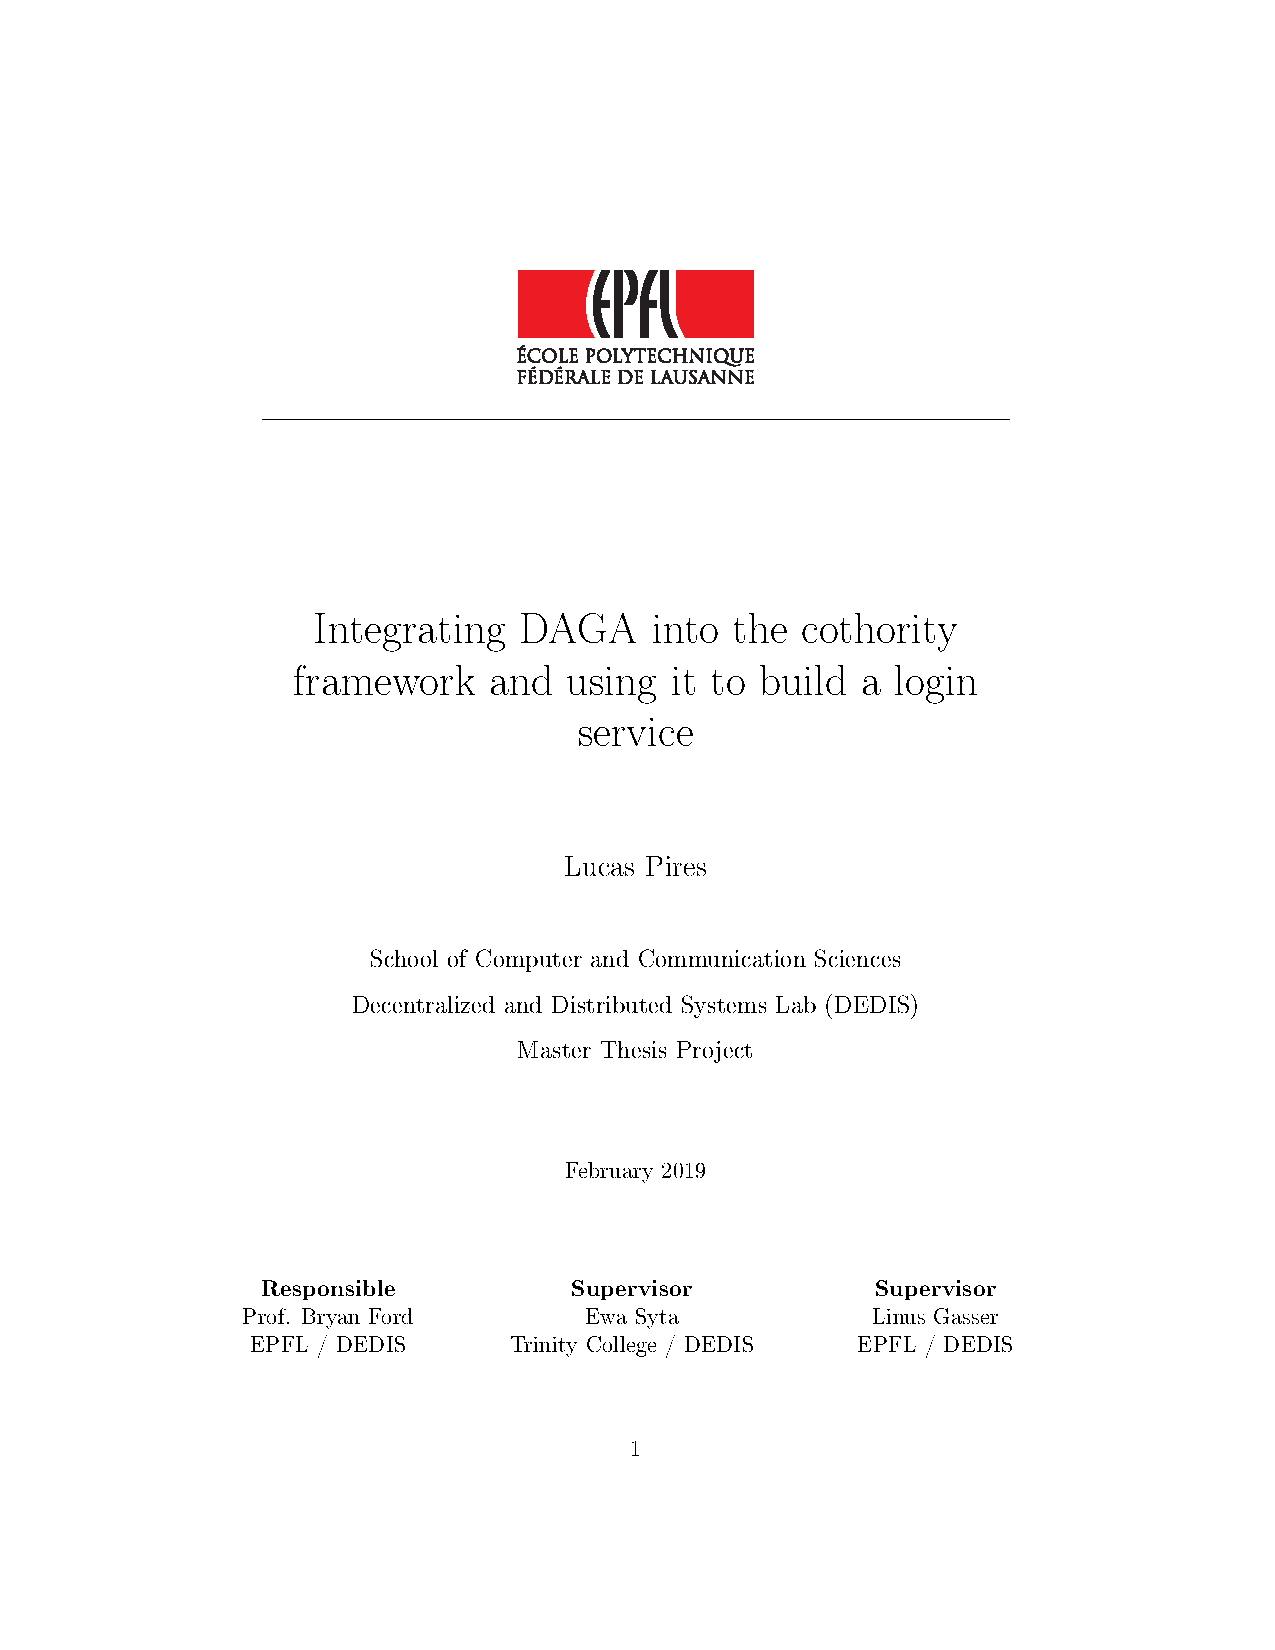
\includepdf{cover.pdf}  % was not happy with input(cover) because I don't know how to format the layout/document class independently for the first page
    \newpage

    \tableofcontents
    \newpage

%    \section{Abstract} % TODO abstract => not...time.. :(
%    % context + motivations + goals + .. previous works + status/contribution etc..
%    \newpage

    \chapter{Introduction}
    \label{ch:introduction}
    \section{Introduction}
In this report, I will present the work that has been done on the CP-MAC cross-platform mobile application. CP-MAC allows a user to use the framework Cothority, developed at the DEDIS lab, in a functional and user-friendly application. The base application containing all the primitives to use the framework was already done during a previous semester project, thus the focus in this project was to improve the user experience and to extend the application with a new functionality. The chosen functionality is the BeerCoin, a long time running joke at the DEDIS lab which consists of beer tokens that can be distributed in a group using Proof-Of-Personhood. A token can then be used to get a beer and the barman can cryptographically verify if this token is part of the allowed group and unused.

    \chapter{Background}
    \label{ch:background}
    \section{Corresponding background}
As CP-MAC aims to provide an intuitive and user friendly interface to access the Cothority framework, multiple technologies have been abstracted into the application to give regular users the possibility to use the application without having to know the inner working of the frameworks it uses. During this project, this idea was kept in mind and influenced the different decisions that had to be made. 

In this section, I will present the different technologies involved in this project and their role in the application. Note that there are several other technologies on which CP-MAC resides that are not described in this section, as they were not implicated in the realization of the project. Thus, if complementary information is needed to understand other specific parts of the application, please refer to the report covering its first implementation\cite{petrimaire2018}. The last part of this section will then focus on the state of the application as it was before the project and which aspects this project have improved. These aspects will then be detailed during the rest of the report.


\subsection{Cothority}
The genesis of the CP-MAC application begins with the framework Cothority, developed by the DEDIS laboratory at the EPFL. The Cothority (short name for \textit{collective authority}) framework provides the necessary components to deploy decentralized protocols over a set of servers, individually referred as a \textit{conode}.  The framework is based on a list of protocols that resolve the most basic challenges of the framework, such as \textit{ByzCoinX\footnote{\url{https://github.com/dedis/cothority/tree/master/byzcoinx}}} that implements the consensus protocol, or \textit{dkg\footnote{\url{https://github.com/dedis/cothority/tree/master/ocs/protocol/DKG.md}}} that implements a distributed key generation protocol. However, in order to use these protocols, Cothority provides services that allows user to communicate with a conode and abstract the protocols. Examples of services are \textit{skipchains\footnote{\url{https://github.com/dedis/cothority/blob/master/skipchain}}}, that defines a permissioned blockchain for storing data, or \textit{cosi\footnote{\url{https://github.com/dedis/cothority/tree/master/cosi}}} that allows a user to get a collective signature of an arbitrary document from the set of conodes.

More generally, a combination of services and protocols defines a Cothority application, which is a high level abstraction to define a useful usage for a set of conodes. The scope is then quite broad, starting from simple command line interface for a specific service to more complex combinations, such as \textit{CISC Identy Skipchain\footnote{\url{https://github.com/dedis/cothority/tree/master/cisc}}}, an extension of the more basic skipchain service that contains, inter alia, a module to handle distributed SSH keys rotation. I will now describe the Cothority application which has been involved in this project, the Proof-Of-Personhood.
\subsubsection{Proof-Of-Personhood}
The Proof-Of-Personhood results from the work done by Maria Fernanda Borge Chavez at the DEDIS laboratory. She proposes a way to solve a known problem on the Internet, which is the ability for a given service to recognize an user without compromising his anonymity, for example if a user is allowed to get only a specific amount of an arbitrary resource but doesn't want to disclose its identity. To achieve this, every member of a specific group gets a token that can be used to authenticate himself towards a service. This will also generate a tag, specific to the user and the service, which can be used to recognize that user (more information about this process is available at section \ref{sec:linkable_ring_signature}: \nameref{sec:linkable_ring_signature}). As the tag will be different among the services, they cannot team up to exclude or identify a specific user. The generation of these tokens is the key topic of her work.

More specifically, two types of actor take part in the generation of the tokens: the organizers and the attendees. Each organizer has a conode, which will be used for the registrations and the cryptographic operations. On the other side, each attendee have their own key pair, which corresponds to a specific identity. This being set up, the following steps can be achieved:

\begin{itemize}
	\item First, the organizers have to define the conditions of a \textbf{PoP-Party}, which is a meeting between all the organizers and attendees. These conditions contain the location, the date, and the list of the organizers' conodes. This is called the \textbf{Party Description}. It has to be the exact same for every organizer, as the hash of the description is used to identify the party.
	\item At the given date and location, every organizer and attendee meet. Each attendee has to pass in front of each organizer to get his public key registered (i.e, adding his public key to the set of all the attendees' public key to later prove that he was present at this party). Of course, some precautions have to be taken to prevent an attendee to register multiple times with different keys. For example, each attendee could be marked with permanent pen while leaving the room, which prevents him to go back in and get registered again.
	\item Once every attendee is registered, the organizers can \textbf{Finalize} the party. The list of public keys is added to the end of the party description, and a collective signature of this file among all the organizer conodes is generated. By combining the file and its signature, we get a \textbf{Final Statement}, which is the necessary material to verify a signed message. In the other side, the attendee combines the final statement with his key pair, which results in a \textbf{PoP-Token}.
	\item Using Linkable Ring Signature (see \ref{subsubsec:linkable_ring_signature}) and PoP-Token, a user can sign a message, which can then be verified by the holder of the final statement.
\end{itemize}

Of course, all of these steps are implemented in the Proof-of-Personhood application of Cothority and can be accessed using an API\footnote{\textit{Application Programming Interface}}.

\subsection{Kyber}
The Kyber library\footnote{\url{https://github.com/dedis/kyber}} is a key element in the Cothority framework. It provides a toolbox for all the cryptographic operations that are needed. Especially, it supports all the algebraic operations on group elements (such as elliptic curve points and scalars), as well as random generators and elements mar\-shaling. It's implemented in Go, but as a lot of front-end applications (such as CP-MAC) require a JavaScript implementation, a partial and develop\-mental port named KyberJS is available. However, it is important to note that some features from Kyber are not available in KyberJS, such as extendable-output functions (see point \ref{subsubsec:blake2} for more information) or (Linkable) Ring Signature (see \ref{subsubsec:linkable_ring_signature}). In this project, a special implementation of the latter has been made as it became necessary for the evolution of the application. Its implementation is described at section \ref{sec:linkable_ring_signature}.
\subsubsection{(Linkable) Ring Signature}
\label{subsubsec:linkable_ring_signature}
Ring signature gives the possibility for a user to sign a message on behalf of a group, in the sense that the receiver of such a message will be able to verify that the signer is indeed a member of the group without revealing who specifically signed it. Here, each group member is represented by his public key. This leads to interesting applications, as the only constraint to create such an anonymity set is to have the public key of each member. For detailed information about the inner working of ring signatures, please refer to the original publication at \cite{rivest2001}.

Kyber also provides the possibility to create linkable ring signatures, which implementation follows the paper \cite{cryptoeprint:2004:027}. The additional property that linkable ring signatures asserts is that two signatures from the same signer can be linked. In other words, a link scope is used during the signing and verification process, then, in addition to the signature, a linkage tag is produced. This tag is unique to the user and to this scope. Thus, given two messages signed under the same linked scope, the verifier of the signature can assert (1) whether the signers are members of the group or not and (2) whether the two signers are the same member or two different ones. A tag can also be used to remember if a specific user have already been "seen" under the current link scope. This application will be particularly useful in CP-MAC. More generally, useful applications can be found for linkable ring signature. For example, different services (Wikipedia, E-Voting, and so forth) could get their own view on a group, without them being able to collude to find out link between users, or to exclude specific users.
\subsubsection{BLAKE2}
\label{subsubsec:blake2}
During the signature and verification process of linkable ring signatures (as defined by \cite{cryptoeprint:2004:027}) a cryptographic hash function is required. In Kyber, this task is handled by the BLAKE2 function. BLAKE2 comes with several interesting characteristics : it's faster than most of the current popular hash function (SHA or MD5) and it's at least as secure as SHA-3 (see \cite{aumasson2014}). BLAKE2 is available in two versions :
\begin{itemize}
	\item BLAKE2b, which produces digests of size up to 64 bytes and is optimized for 64 bits processors
	\item BLAKE2s, which produces digests of size up to 32 bytes and is optimized for 32 bits processors
\end{itemize}

\subsubsection*{Extendable-output functions}
BLAKE2 also offers the possibility to generate extendable-output functions (XOFs) from each variants of BLAKE2, respectively named BLAKE2Xb and BLAKE2Xs. A XOF allows generating digest of arbitrary length (although there is a limit of 256 GiB for BLAKE2Xb and of 128 GiB for BLAKE2Xs), which is especially interesting to create deterministic random bit generators (DRBG). In Kyber, both of BLAKE2 versions and their respective XOF are implemented and BLAKE2Xb is used in the computation of ring signatures. However, these XOFs have not been ported yet to KyberJS.

\subsection{CP-MAC}
As CP-MAC has already been extensively presented in \cite{petrimaire2018}, I will rather do a quick overview of the application and then focus on the state of the application as it was before the beginning of this project. This will then allow me to present the road map of the execution of the project to underline the components of the application that have been improved.

CP-MAC implements a simple interface to use two major applications of the Cothority framework : the Proof-Of-Personhood and the CISC Identity Skipchain. However, these are services that are though to use for a non-experimented user who doesn't have access to an easy-to-use front-end. CP-MAC tries to resolve this problem by combining the mobility offered by a smartphone application with a  more intuitive user interface than CLI\footnote{\textit{Command Line Interface}}.

\subsubsection*{NativeScript}
Under the hood, CP-MAC is made above the NativeScript framework, which allows developing a native cross-platform mobile application in JavaScript (for the application logic), XML (for UI elements) and CSS (for UI styling). It is a great advantage, as styling an application on NativeScript is essentially the same as styling a website, apart from some exceptions. The vast majority of CSS attributes are available, even some advanced ones, such as animations. Also, on both platform, NativeScript allows calls to native APIs such as \textit{Time} on Android, or \textit{UIAlertView} on iOS. It's then possible to manipulate directly those objects from the JavaScript code. 

Also, NativeScript gives the possibility to create Plugins, which are native pieces of code with a common JavaScript interface. For example, one could develop advanced Plugins such as Web Sockets or Fingerprint Authentication that have their specific native implementations on iOS and Android, but that will be manipulated through a single object in JavaScript. 

It's however important to note that NativeScript does not directly compile JavaScript to native code. Instead, it uses the power of JavaScript virtual machines to inject global objects representing the native APIs, that are then used to intercept native calls and let NativeScript Runtime redirect them to the native libraries. Apart from that, the application logic is executed in JavaScript by their respective engine, i.e \textit{V8} on Android and \textit{JavaScriptCore} on iOS\footnote{as of June 2018}.




    \chapter{Implementation}
    \label{ch:implementation}
        % don't forget to see if I forgot ideas and paper see zotero, quotes etc.
    % don't forget to see if everyhting present, see other notesfiles.txt
    % follow the desicion processes documented in worksheet
    % keep title in worksheet as things that worth a word in report !

    %TODO see if need to add something and crossref
    The following chapter will present the work that was done during the project the design choices and the current state of advancement.
    We begin by describing the goals and current state before detailing the work done on the three main parts of the project individually:
    \begin{enumerate}[leftmargin=!,itemsep=-1ex]
        \item the DAGA library (see~\autoref{subsec:library})
        \item the DAGA cothority service (see~\autoref{subsec:cothority})
        \item the login service and the proof of concept (see~\autoref{subsec:loginservice})
    \end{enumerate}

    The first part uses the work from a previous student as a starting basis\sidecite{villard_report_pfs_pop.pdf_2017},
    the second part builds on the previous to integrate DAGA into the cothority framework,
    while the last part makes use of the previous parts and CoreOS's dex project\sidecite{noauthor_announcing_nodate}
    to implement a login service.

    \section{Overview and goals}
    %TODO cross-ref with future/results/background/previous work
    As already mentioned in the introduction\sidenote{\autoref{ch:introduction}}, the final goal of the project is to offer
    \emph{DAGA authentication as a service}\sidenote{or a "login service" as put in the title}.
    We aim at letting current and future system designers leverage easily DAGA's promises in their design and thus
    offering them the opportunity to take more into account the privacy of their end-users whether it is critical for their mission or not.
    As hinted we would like our solution to remain as generic as possible, i.e.\ not tailored and tied to particular uses
    cases and deployment scenarios.
    Naturally we will need to keep the properties\sidenote{see~\autoref{subsec:properties}} of DAGA while doing so and we will
    try to separate as much as possible the different components and building blocks into well defined abstraction levels.\sidenote{
        e.g.\ to build the "login service", everything from the DAGA library to the full cothority service, looks just like
        a "simple" authentication primitive:\newline \(yes;tag|no;0 = daga(request)\)
    } This implies too that we would like to not pollute the created lower level primitives (e.g. DAGA cothority) with the
    requirements of the upper ones (e.g.\ login service) while implementing them, and thus offering them untouched for other
    future usages.

    \section{Current state and contributions}
    As part of the current work the following contributions were made:
    \begin{itemize}
        \item the DAGA library was ported to kyber.V2, the client-side code was rewritten, issues have been identified and some fixed,
                documentation as well as guidelines for the rewriting of the server-side code have been added.
        \item the library was used to implement DAGA in the cothority framework, featuring:\newline
            \begin{itemize}
                \item a new \emph{service} allowing to build cothorities supporting DAGA authentication and the creation of DAGA contexts
                \item three new \emph{protocols} to support the service
                \item a CLI app to interact with it
                \item test coverage edging 80\% for the protocols and service
                \item boilerplate allowing to run simulations locally as well as on DETERLab's testbed facilities
                \item compliance with the tool that generate proto files to allow future interop with other languages
            \end{itemize}
        \item a system allowing 3rd-party services to delegate the authentication of their users (through the well established OpenID connect standard)
            to a running DAGA cothority was implemented.
        \item working, reproducible and customizable proof of concept of the system mentioned above
    \end{itemize}

    \section{Building blocks / Components}
    \label{sec:components}
    As said, the project can be divided into three main and reasonably well separated level of implementation, or components.
    This section will describe them in turn.

    \subsection{DAGA library}
    \label{subsec:library}
       
    This part builds upon the work of a previous student available on Github.\sidecite{villard_deniable_2017}
    The library is implemented in golang\sidecite{pike_go_nodate} and uses heavily the Kyber
    cryptography library developed at EPFL by the DEDIS team\sidecite{dedis_advanced_nodate}.\newline

    The goal of this part of the project was to ultimately integrate the new DAGA library into Kyber.
    The previous work was first ported from kyber.v0 (Crypto.v0) to kyber.v2, before being reworked to address some issues.\medskip

    Since the goal was to integrate the library into Kyber and that one of the main point of Kyber is to \blockquote{
    facilitate upgrading applications to new cryptographic algorithms or switching to alternative algorithms
    for experimentation purposes}\footnotemark[\thefootnote]
    we decided to try to leverage as much as possible of the facilities offered by Kyber.

    The first step in this direction was the addition of a new Suite\sidenote{
        A Suite is \blockquote{
            an abstract interface to a full suite of (\ldots) crypto primitives chosen to be suited to
            each other and have matching security parameters.
        } quoted from \href{https://github.com/dedis/kyber/blob/v0/abstract/suite.go}
    } interface for DAGA, that will notably allow future users to switch to other cryptographic building blocks if needed or wanted.
    For instance the original paper  worked in a Schnorr group\sidenote{
        specifically, the group of quadratic residues modulo a safe prime.
    } (i.e.\ a large prime-order subgroup of the multiplicative group of integer modulo \(p\) where \(p\) is prime),
    while the previous and current work implementation works with a prime-order group constructed with the twisted Edwards curve birationally equivalent to
    Curve25519\cite{yung_curve25519:_2006}(i.e.\ the suite uses the same group that is used in Ed25519's variant of the EdDSA signature scheme).

    We can see that from DAGA's perspective either implementation is fine as long as it satisfy DAGA's assumptions on the
    algebraic group being used, which is the case.\sidenote{
        DAGA is heavily based on discrete logarithm cryptography,
        thus DAGA assumes a group \(\mathcal{G}\) where the decision diffie-hellman problem\cite{boneh_decision_1998}
        is assumed to be hard (DDH assumption).
    } But from an engineering perspective this means we need to identify the individual high-level operations that are needed by DAGA
    and that would need to be dealt with different level of care depending on the underlying group and primitives used and their implementation in Kyber.
    (e.g.\ for diffie-hellman key exchange, we usually need to validate the public keys.\sidecite{valenta_measuring_2017}
    but with current EC concrete implementation we, at least in theory, don't need to care)\sidenote{
        In the current curve if the secret keys are correctly generated to be multiple of 8 (the curve's cofactor) then
        we don't have to check if the remote public key is in the correct subgroup, because even if it is not,
        the DH shared secret cannot leak (by construction) any bits of the targeted secret key.
        However in practise it is not the case, we noticed that the code generating the secret keys in Kyber is, at the time of writing, not correct,
        still seems that it is not a big deal because I am under impression that bad Points are rejected / not representable
        by the library. % when I think of the amount of time I dedicated to these crypto issues and that I'm just writing shit by lack of time and energy...:(
    }\medskip % TODO if not used to make link with lowlevel crypto concerns maybe dont mention it at all

    As a second major step we can mention, the rewriting of the client-side code and notably the PKClient proof\sidenote{
        see section~\ref{subsubsec:dagaauth}
    } related code to make use of the existing kyber.Proof framework instead of rewriting whole proof machinery by hand.

    This was done for multiple reasons, readability and maintainability for a start, it lessen the bug surface, i.e.\ we only need
    to look for proof related code at one well written, tested and documented place (the kyber.Proof package).
    Then we can view the same rationale from another perspective, since the proof framework is part of Kyber and we eventually
    want to integrate DAGA into Kyber, we might give a try at the "eat your own dog food" motto and use it in our own projects.
    To expand on this topic, we had to design some API wrappers around the proof framework to interface with it in a more
    easy and familiar way.\sidenote{
        see the clientProverCtx, clientVerifierCtx and their methods in client\_proof.go.
    }
    Those wrappers could maybe be adapted into an additional reusable API/pattern for the proof framework to ease future
    usage where, like in our case, the user needs to build interactive proofs across different machines.\sidenote{
        they allow to synchronize easily with a running proof.Prover, to extract the commitments in order to forward them elsewhere,
        then to continue the proof once a challenge was received from the remote end, etc.
    }

    Finally we introduced more documentation with links to original DAGA paper, better error messages and minor refactoring to
    make the code more readable DRY and idiomatic.\newline
    Still in our opinion the server side code is not production ready, nor of same quality level as the remaining of Kyber
    and thus should be mostly rewritten too (including the server proofs).
    This has not been done because the implementation was good enough for our current goal and we moved
    on the next phases in order to not lose more time on it.
    The library is well tested but the tests are mostly unmaintainable and it would be easy to miss some important cases.
    They were refactored to introduce the proper usage of testify and to fix some easy things but they were ultimately left in
    the state they were found.
    This leaves the library in an unfinished state and for all of these reasons and the fact that I don't fully endorse it
    in its current state the integration in Kyber was not performed.\sidenote{
        at some point after the port to kyber.v2 a WIP pull request was made and ultimately closed for the same reasons.
    }
    Still the code is full of comments detailing the direction to take to resolve the situation.


    % TODOs maybe if time and relevant => probably not
    %    -list some of design choices, such as interfaces (client server etc..)to allow multiple concrete implementation in user code (that need other things than pure daga)
    %      list example of benefit and usage ? favorized instead of struct to allow eaysier testing etc (functions accept interface) follow best practises


    % conclude with the fact that I thought about lots of corner cases and implementation issues and identified things that I'd like to see be done but not time
    % -add validations etc.. try to implement recommended practises regarding DH to try to avoid confinements and small subgroup attacks => nope i don't have the energy...


    %-IMO not sure daga should be put in kyber (and for sure not in sign/daga...) its a thing built with kyber but..


    %-since currently there there are no schnorr group in kyber and such schnorr group implementation is likely to be more costly
    %maybe the whole suite idea is finally a bad idea and maybe integrating daga in kyber is a bad idea too


    % had to go for the best given time constraints etc..
    % at some point was told that it is not my job (not very clear from start and divergent opinion of my two supervisors)
    % and more importantly that I won't have time to do the rest if I continue rewriting daga (which we all aggree i'd say)
    % (already huge amount of work, sic syta etc..even if not totally acknowledged by linus that is disapointed I didnt do more (how ???)
    % that's why the work is kinda left in an unfinished state with lots of comments and todos

    % pfff :(


    \subsection{DAGA Cothority}
    \label{subsec:cothority}
        % mostly DONE exept 2 TODO , address when writing future and conclusion!

    This part uses the previously introduced library to implement DAGA in the cothority framework\sidecite{dedis_scalable_nodate}.
    \newline\noindent
    Cothority is a DEDIS project that \blockquote{
        provides a framework for development, analysis, and deployment of decentralized, distributed (cryptographic) protocols.
        A given set of servers running these protocols is referred to as a collective authority or cothority.
        Individual servers are called cothority servers or conodes\footnotemark[\thefootnote]
    }.%\newline
    The following figure depicts an high-level overview of the new DAGA cothority that will be subsequently
    described.
    \begin{figure}% or marginfigure scale=0.45/or reduce cothority and give more room to part below
        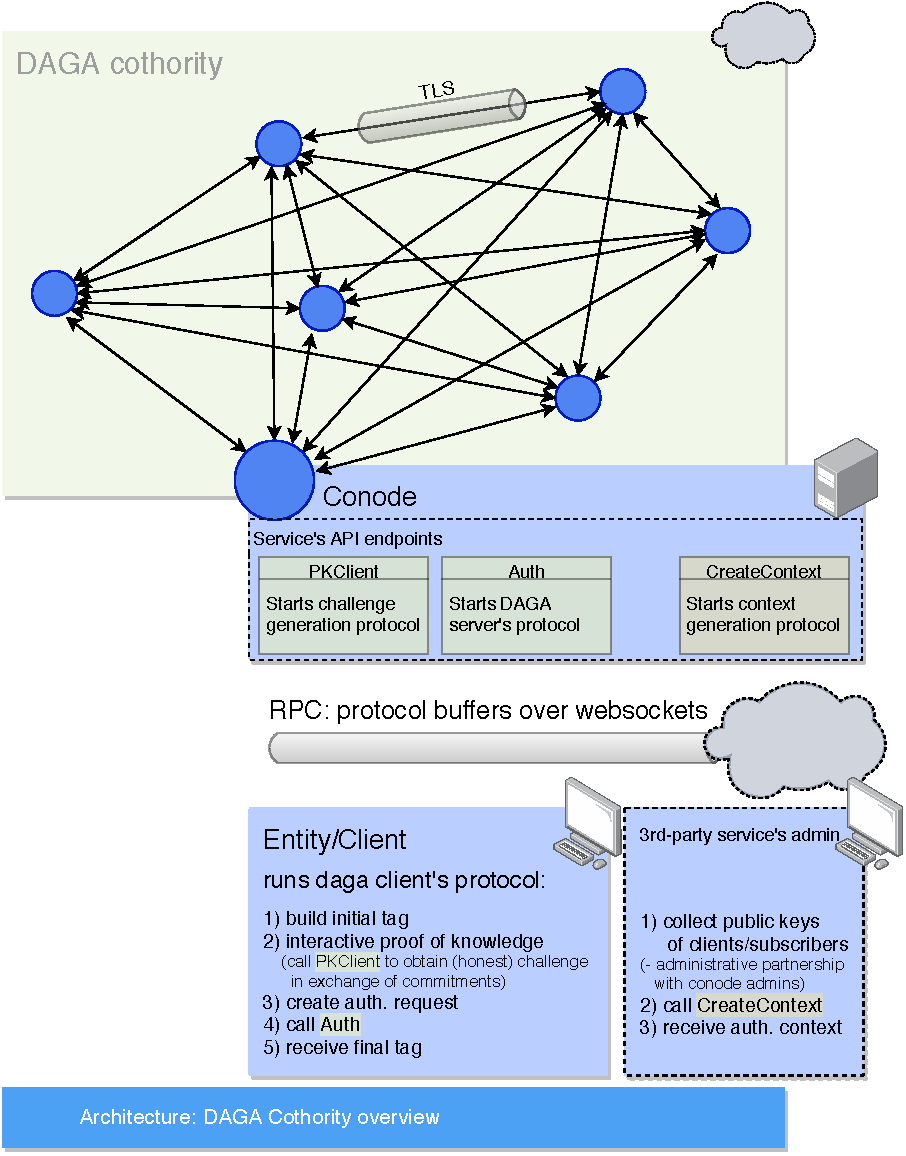
\includegraphics[scale=0.7]{images/dagacothority.pdf}
        \caption{high level overview of DAGA in the cothority framework}
        \label{fig:dagacothority}
    \end{figure}

    \subsubsection{Context Creation}
    As said in the background chapter, every party needs to have access to a public (in the "not sensitive" sense)
    authentication context\sidenote{see section~\ref{subsubsec:dagacontext}} before being able to do anything.
    To create such context, the protocol described in~\cite[Sect.~4.7.3]{syta_identity_2015} was implemented. % TODO stress somehow that this is new ?

    A client can (typically an admin of a 3rd-party service)
    create a context by:
    \begin{enumerate}[leftmargin=!,itemsep=-1ex]
        \item Gathering the long-term public keys\sidenote {
        To do so it is envisioned to offer tools allowing to scrap them out of a POP\cite{borge_proof--personhood:_2017}
        party transcript for instance,
        but the admin is free to collect them by any mean that fits its agenda.
        } of the \emph{group} members (or entities, typically the subscribers of the service).

        \item building a cothority by establishing individually and administratively partnerships with the admins that run
        DAGA enabled conodes. (but we can imagine "open access" conodes) and creating a roster\sidenote{
        a structure describing basically how to reach them and communicate securely with them (public keys)
        } out of the  process.

        \item finally sending an authenticated CreateContext request (containing the keys and roster) to a random conode in the roster.
    \end{enumerate}

    Then the conode receiving the request checks first if it has a matching partnership before initiating a new instance of
    the context generation protocol, with the other nodes listed in the roster as partners.
    During the protocol run, all other conodes will check in their turn if they accept the request before acceding to the
    request of the leader and helping it building the context.
    At the end of a successful protocol run (where nothing strange has been detected by any node), the new context is sent
    back to the client and every node will start serving the newly created DAGA context.\sidenote{
    or said differently, accepting authentication requests under the context, and hence establishing effectively a new
    \emph{collective authority} for the context by doing so.
    }

    \smalltitle{Current state:}
    As currently implemented, each conode can serve multiple different contexts at once
    (each with possibly different daga server identities/public keys)
    % TODO ? one key one purpose, dissociate daga service from conode/onet internals choices of keys etc..
    % node-node channels are authenticated using keys in roster which is tied to authentication context
    and at the end of each context creation the state is persisted in
    a bbolt database, allowing a node to retrieve it after a potential shutdown or crash without destroying permanently the cothority
    and/or forcing everyone to rebuild a context.

    However there are currently no facilities/boilerplate to manage and conduct the administrative partnerships that was mentioned in the
    described scenario nor to authenticate the 3rd-party services admins, hence currently the conodes are "open access" DAGA nodes.
    Still the service and protocol were implemented while keeping those ideas in mind and already have places to check such things,
    making the addition straightforward.\sidenote{
        Have a look at the dagacothority/service/service.go
    }
    One of the ideas would be, interestingly, to reuse DAGA for that purpose, we can imagine that we define administratively/offline a
    context whose members are the people that have a partnership with the conode that allow them to create contexts (~similar to authenticated darcs).
    Then a running cothority (serving the context) and containing the conode, authenticates the request.
%    => the node is convinced that the "remote now anon 3rd-party service admin" has the right to create new contexts
%    => (+) KISS, can use only DAGA, no need to use alien protocols and things like openPGP or DARC management etc..
%    => (+) ~"eat your own food" preserve 3rd-party admin privacy, don't throw out of the window our own goals and advices on the separation of authentication and identification etc..
%    => the thing now becomes: offering ways to manage the partnerships and setup those partnership contexts.
%    chicken and egg problem but now we can decide to bootstrap them differently using whatever means we want
%    (a cli app ? + administrative context loaded from known location at setup time)

    %TODO ref% FIXME cross ref to Future where I'll talk about the things envisioned for the auth. !!

    As seen the DAGA cothority was designed such that every conode retains completely its free-will,
    each conode is independent and tied only by the contexts it serves to form possibly multiple cothorities with possibly
    different partners.
    Finally quoting~\cite{syta_identity_2015} those DAGA enabled conodes are expected to be \blockquote{
        deployed by a federation of organizations wishing to support responsible forms of anonymous participation (...),
        anonymity system providers such as the Tor project, non-profit organizations whose aim is to further online privacy
        and anonymity, or even for-profit organization desiring strong guarantees and large anonymity sets for their clients.
    }

    \subsubsection{Authentication and \(\Sigma\)-Protocol}
    \label{subsubsec:sigmaprotocol}

    A client having in possession a suitable authentication context
    can authenticate itself to the DAGA cothority by sending its authentication message to the \emph{Auth} endpoint of a random conode.

    As already described in section~\ref{subsubsec:dagaauth}, to build such an authentication message, the client
    has to conduct a zero-knowledge proof of knowledge with the cothority at the verifying side.
    To do so it will call the \emph{PKClient} endpoint of a random conode to request a challenge in exchange of commitments.

    Since the proof in question is of the \(\Sigma\)-protocol kind, the zero-knowledge property\sidenote{
    and hence the anonymity and deniability properties of DAGA
    } holds only if the verifiers (thus the challenge) are honest\sidenote{(special HVZK property)}.
    Hence we need to have the servers \blockquote{
    collectively generate \(c_s\) [(the challenge)] so that each server, which would include at least
    one honest server, contributes its randomness towards \(c_s\).
    }\cite{syta_identity_2015}
    Moreover if the prover can predict the challenge (maybe with the help of some dishonest servers),
    it will allow it to cheat by crafting its first move (the commitments) using the verification formula
    or put differently, by abusing the HVZK proof structure and using the "simulator + rewind verifier" approach.
    % TODOs, check what aboout the space of the challenge, remember having read sommewhere that it should not be too large
    % for the ZKness to hold...=> if thats the case then here is a shady thing in daga

    \noindent
    To summarize the distributed challenge generation protocol has two main purposes:
    \begin{enumerate}
        \item the obvious one : make the "verifier"(cothority) honest to keep the proof zero-knowledge.
        this is solved by the fact that we assume an anytrust setting, at least one honest server will contribute its randomness to the challenge.
        \item the less obvious one: convince individually the servers that the challenge is honest
        (they trust themselves to add their randomness to it) and that the client and other servers cannot collude and cheat.
    \end{enumerate}
    Hence at the end both the honest client and the honest server are ensured of the randomness and "honesty" of the cothority as a whole.

    % TIE to commitments, state etc..
    Additionally, the proof being interactive\sidenote{in order to offer the deniability property of DAGA},
    it convinces only the participants.
    As a consequence, if the servers want to verify it later (Auth endpoint) based only on the transcript embedded in the authentication message\sidenote{
        That's how DAGA is described in~\cite{syta_identity_2015},
    }, additional care and mechanisms should be put in place.
    Indeed if nothing is done (as it was the case with the previous implementation\cite{villard_deniable_2017}) the prover
    can cheat using the same technique described above.\newline
    There are two approaches to prevent this from happening:
    \begin{enumerate}
        \item keep state (commitments and challenge) between the \emph{PKClient} and \emph{Auth} requests at each node,
                and rely only on it to verify the proof.
                This approach was chosen by~\sidecite{wolinsy_daga_2014}
        \item or avoid by following the "keep state in clients" motto of RESTFul services.
    \end{enumerate}

    We chose the second option, and implemented it by having the servers tie the challenge to the commitments by
    each issuing a signature on \(challenge||commitment\) instead of only challenge at the \emph{PKClient} step.
    This way, when the client calls later the \emph{Auth} endpoint, the servers can individually verify that the challenge
    and commitments have not been altered by verifying their own signatures\sidenote{
        the signature ties the challenge to the commitments and at the same time protects authenticity and integrity of the pair
    }.

    % TODO ? - verifier extracting secret, would be the right place, ...
    %(if proof run 2 times with same commitments, i.e. abusing special soundness proof, using "extractor + rewind prover" approach => PRNG must be properly setup !!)
    % careful with rndgen, special soundness property allows people with 2 transcripts such as as malicious server to extract
    % client secret key (only if prover rewound,  same t ==> means need to be sure that random properly working !! => care in cloud setup if not proper source of entropy)
    % this is done correctly by using golang's crypto.rand that should do the job

%    % FIXME: here with new title thoughts/etc. or future/conclusion, see when writing future
%    TODO
%    at one point I investigated the possibility to use randherd to generate the challenges
%    => not done because :
%    1) time, first simpler min viable approach
%    2) add a dependency to daga, tie to implementation in cothority framework => need to maintain 2 things (kyber daga need to have things related to building challenge)
%    3) not sure how to tie the resulting challenge to commitments in a way that convince everyone that nobody is cheating
%    see later, now each server signs cs||commitments at the end (and is convinced is random by construction, add his own randomness)
%    but at the end of randherd, client of randherd call (say leader of daga challenge generation)
%    obtain decentralized honest publicly verifiable randomness ? but how can we tie it to the commitments at all servers ?
%    say that it is the client while building proof that request the challenge via randherd (same cothority for randherd + daga)
%    as before problem is servers' don't have a chance to tie the challenge to the commitments to prevent prover cheating (see proof)
%    => fallback to first option manage request state in servers
%    since time was short, idea dropped/postponed




    \newpage

    \subsection{Login service}
    \label{subsec:loginservice}
    
    This part will describe the designing of the login service's architecture.

    \subsubsection{Intro, problems, options}
    Up to now we have a running DAGA cothority service that can authenticate clients.\sidenote{
        see Figure~\ref{fig:login0} below.
    }
    Now we want to introduce a 3rd actor in the picture, a service provider that want to use the running DAGA cothority to
    authenticate its end-users on its behalf.
    We already implemented facilities to create authentication contexts out of a list of public-keys, remains now to
    introduce a communication protocol between the three actors that allow for such delegation while preserving
    DAGA properties.\sidenote{
        notably deniability, which as you will see is not that easy. % TODO keep ?
    }

    % standard high level view of auth. delegation
    Figure~\ref{fig:signin} shows a typical authentication delegation flow and introduce the classical terminology that will be used throughout the chapter.\sidenote{
        it was adapted from a figure present in a really good blog post~\cite{vibro_oauth_2013}
    }
    \begin{figure}
        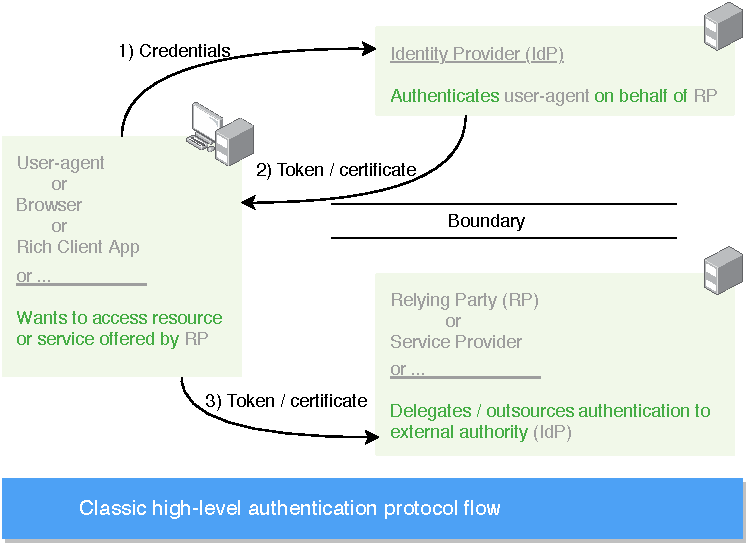
\includegraphics[width=\linewidth]{images/signIn.pdf}
        \caption{Classic high-level authentication protocol flow}
        \label{fig:signin}
    \end{figure}

    %auth delegation problems and necessity,
    Authentication delegation mechanisms are necessary since in all complex systems, we cannot ask every players that provide
    access to services or resources to deal with the management of identities and authentication as well.

    Additionally, while it is true that in theory DAGA can be used anywhere as an ideal replacement of linkable
    ring signatures (LRS) schemes with the added benefit of deniability and forward security\cite{syta_identity_2015},
    the replacement is not straightforward in practise.
    In the LRS case everyone can verify the signature whereas in vanilla DAGA only the cothority is convinced
    of the user authentication\sidenote{and only at the time of verification if there are no other session mechanisms in the picture}
    and the result of the process is only a linkage tag / pseudonymousID that is to be considered public since all the servers
    have access to it.

    The only remaining option, as hinted, would be to require that services interested into using DAGA as authentication mechanism
    be part of the DAGA cothority.
    Not only this is not practical for complex systems, but we would need to either modify the current DAGA cothority code
    to accommodate for such scenarios (e.g.\ provide hooks etc.) or tolerate having specialized version of DAGA nodes for each application.
    Finally this would imply that we are mostly done since the remaining work would be to implement such tight integration mechanisms,
    which is meaningless without having well defined specifications for the services requirements.

    Hence if we want to be as generic and simple as possible and not restrict ourselves with such specific design,
    we need to think of ways allowing to delegate authentication, i.e.\ ways allowing the user-agent to authenticate to the 3rd-party
    with the help of the DAGA cothority.

    \smalltitle{Strawman designs, options}
    To visually represent what has been said above and develop further the options facing us, we start from the following situation:
    \begin{figure}
        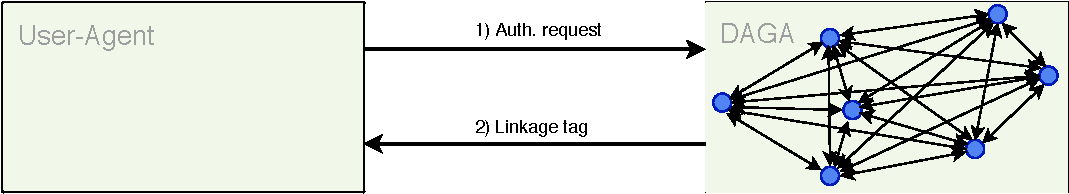
\includegraphics[width=\linewidth]{images/login0_daga.pdf}
        \caption{basic no delegation scenario}
        \label{fig:login0}
    \end{figure}

    As a first way to address the problem mentioned above, we can do the following (for instance):
    \begin{figure}
        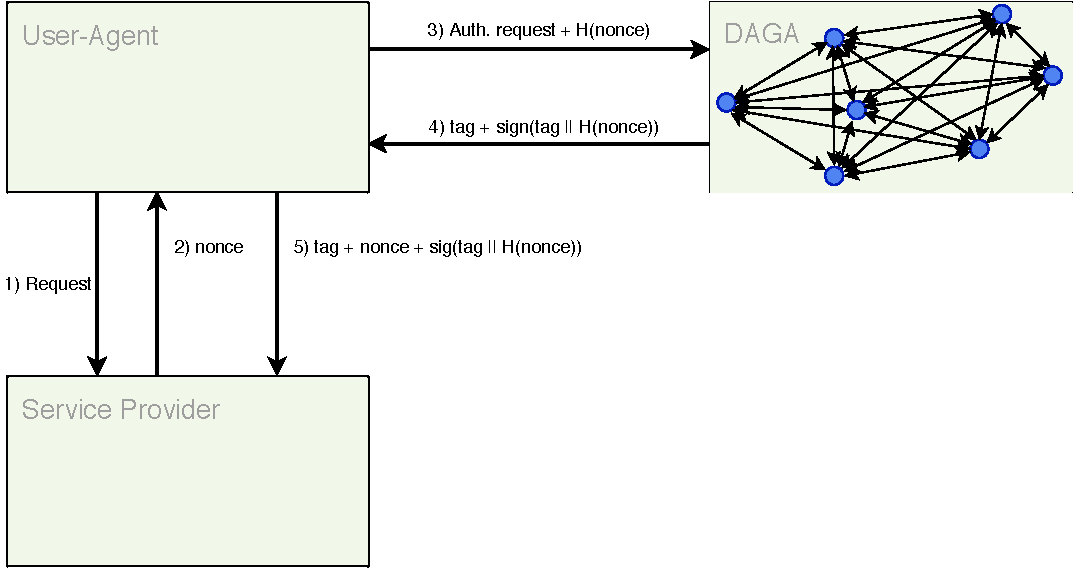
\includegraphics[width=\linewidth]{images/login1_daga.pdf}
        \caption{adds a way to convince 3rd-party that user-agent authenticated with the DAGA cothority}
        \label{fig:login1}
    \end{figure} % TODO modify fig, add explanation for signature in picture, + verification

    But now we just modified the DAGA cothority to make it handle nonces and conversely this requires to closely tie the 3rd-party services
    sign-in code to the DAGA case.
    Another hidden assumption here is that the 3rd-party service has access to the user assets, effectively we put it in a position
    where it can authenticate itself as the user-agent to any authorization mechanism pipelined behind.
    Hence we just restricted ourselves to specific use cases s.t.\ forums or wikis.\newpage

    To address the mentioned issues, we can do the following:
    \begin{figure}
        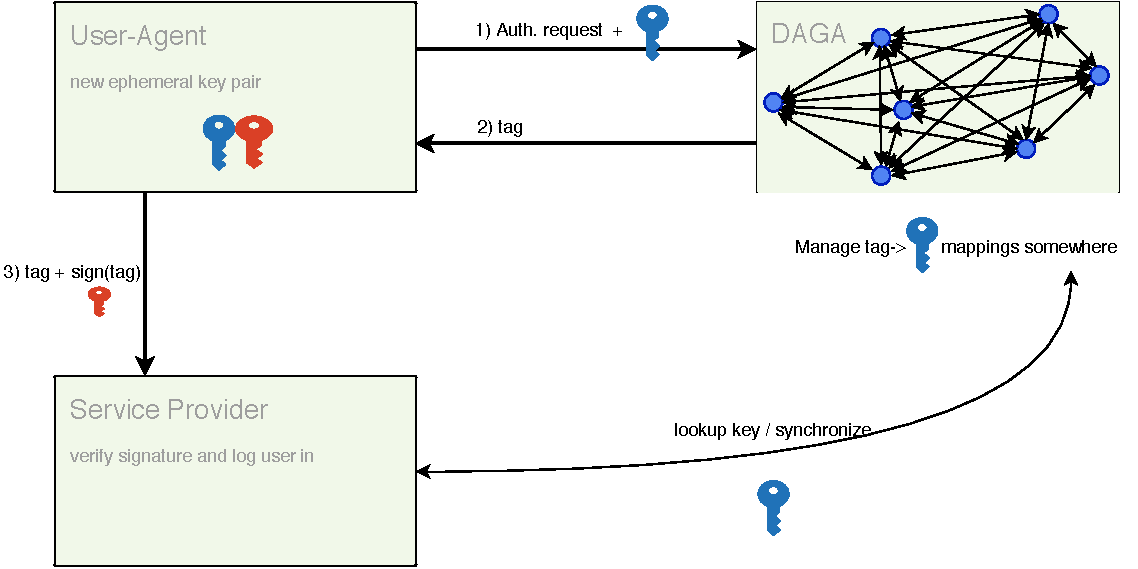
\includegraphics[width=\linewidth]{images/login2_daga.pdf}
        \caption{adds a better way to convince 3rd-party that user-agent authenticated with the DAGA cothority}
        \label{fig:login2}
    \end{figure}

    This is essentially what was described in~\cite[Sect.4.5.1]{syta_identity_2015} and what was done by the dagas
    implementation\sidecite{wolinsy_daga_2014}.
    With each successful authentication the user-agent has the opportunity to register with the cothority a new ephemeral public key
    that is not tied to its long-term ID / public key but to its linkage tag / pseudonymousID\@.
    Furthermore, now the service provider doesn't know the ephemeral secret key and thus cannot authenticate itself as the user-agent.
    \newline
    This is already better than the previous designs since now the cothority is almost not modified, we only need to introduce an additional
    "key server" role that can be implemented in different non-intrusive ways to the cothority implementation\sidenote{
        (e.g. cothority can just publish \(tag \mapsto key\) mappings on a public key-value store etc.)
    }.
    \newline
    However as a new downside we just lost forward-security and deniability, if client's ephemeral secret key is ever compromised we can retroactively
    compromise its anonymity in all past exchanges, since we are now convinced that only it could have issued these signatures.
    In fact looks like we just transformed DAGA into a LRS scheme offering the possibility to rotate keys as a bonus.
    To mitigate this issue we can use very short lived keys etc..
    Additionally we would need to make sure too that any conode processing the request cannot replace the key
    with one under its control.\medskip

    %obvious, interesting but ..offtopic
    %Using the same idea we could even transform the DAGA cothority into a "Deniable Anonymous Group Database" where instead of
    %registering keys the group member can manage some data etc..

    Up to now, all the described approaches are still somewhat home-cooked and not readily interoperable with existing systems
    deployed in production.
    If we want to go down that path and still interface easily with existing systems we would need to provide bridges or
    connectors, one of such option is to provide authentication strategies for well established authentication middleware.
    e.g.\ passport.js, accounts-ui or omniauth for respectively the node.js Meteor and Rails web app worlds.\medskip

    The next and last high-level option we will describe essentially just looks like Fig.~\ref{fig:signin} (see in margin) that introduced
    authentication delegation.
    \begin{marginfigure}
        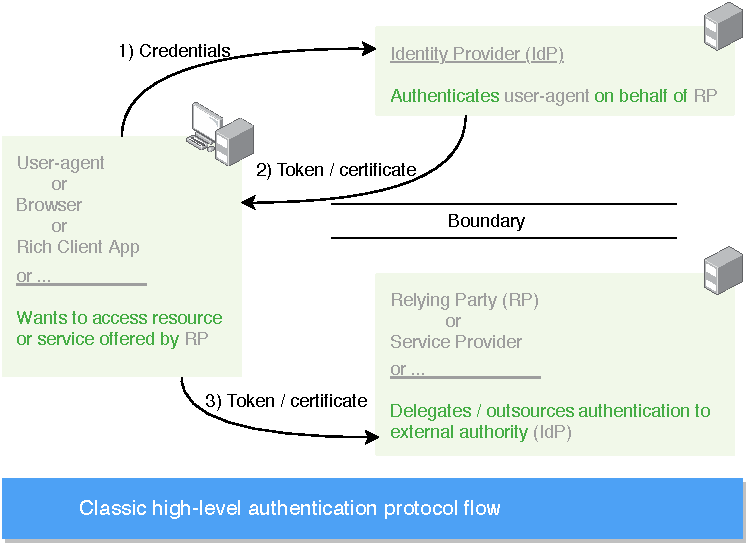
\includegraphics[width=\linewidth]{images/signIn.pdf}
    \end{marginfigure}
    \begin{figure}
        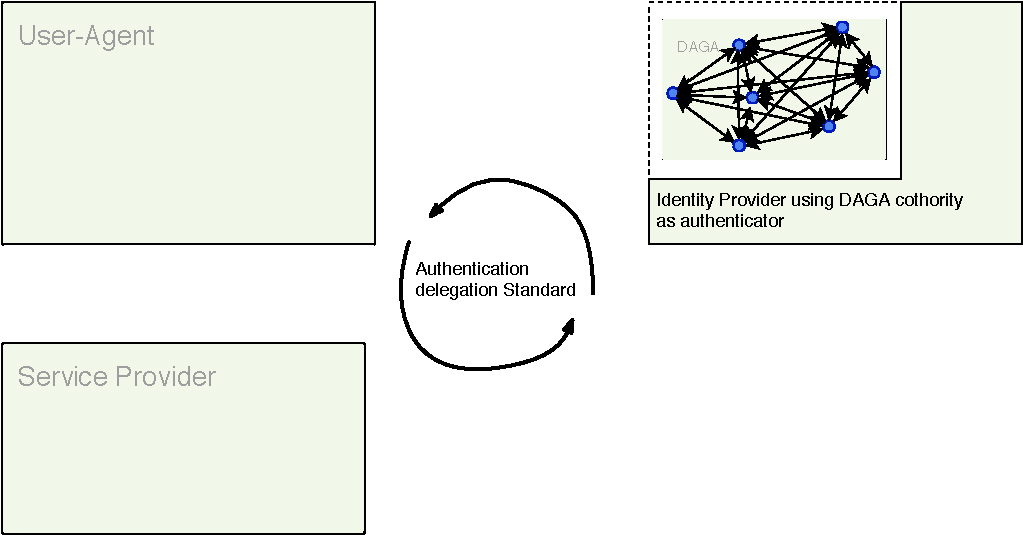
\includegraphics[width=\linewidth]{images/login3_daga.pdf}
        \caption{introduce new trustee entity (IdP) and uses standardized ways to convince 3rd-party that user-agent authenticated with the DAGA cothority}
        \label{fig:login3}
    \end{figure}
    In Fig.~\ref{fig:login3}, instead of reinventing the wheel we rely on existing and well proven protocols and standards for authentication delegation.
    It is the easiest way to have something working quickly and correctly\sidenote{
        designed with care and over time by people and industries that are experts in the field.
        % And thus a design rushed in 2-3 weeks as part of an unrealistic academic project with laughable deadlines cannot compete
    } that would offer us the additional benefit to interface easily with existing services that most definitely already use those mechanisms
    in their authentication workflow.
    To do so we need to introduce a new actor in the picture, the IdP that will use the DAGA cothority as authentication primitive.

    \subsubsection{Chosen solution and PoC}
    Now that we discussed the importance to use an authentication delegation system and exposed different options,
    we need to choose how to implement such system and how it will be used in our PoC\@.
    From the decision keys introduced in the previous description, we chose to use the last option, and we fixed the
    authentication delegation protocol to be OpenID connect.

%    \smalltitle{Background}
    OpenID Connect\sidecite{coreos_openid_nodate} (OIDC) adds an identity layer to, and build upon, the well known OAuth 2.0 authorization framework.
    It is one of the major standard for authentication in the modern world.
    The other choices of framework could have been \emph{SAML}\sidenote{
        Security Assertion Markup Language
    } or eventually Kerberos in controlled environments.

    To build our IdP we chose to use the free-software dex OIDC identity provider which is written in Go and maintained by the CoreOS project.

    Fig.~\ref{fig:poc} describes the system we designed to power the PoC.\
    \begin{figure*}
        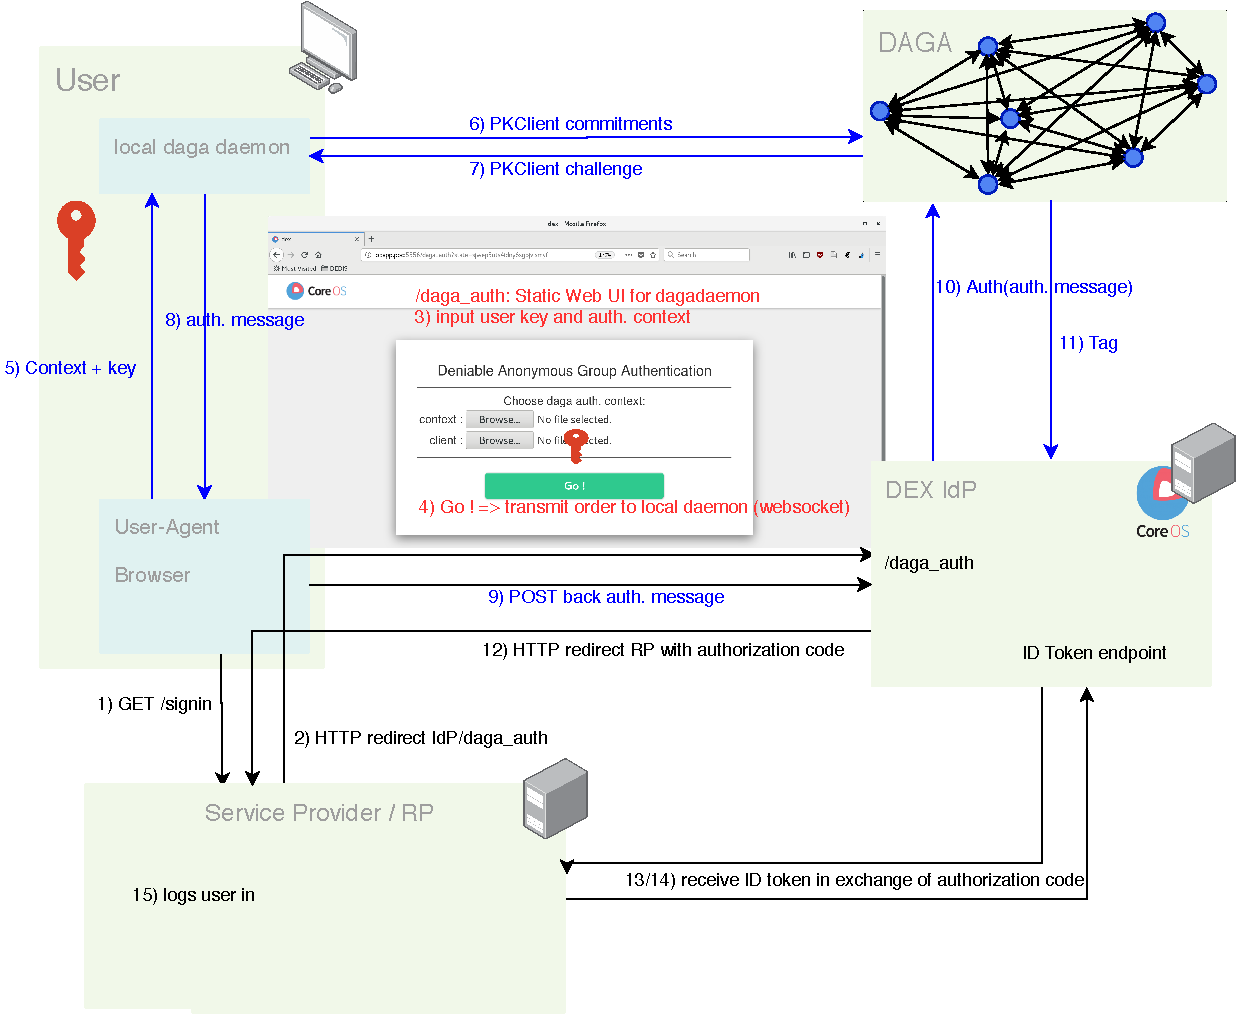
\includegraphics[width=\linewidth]{images/poc.pdf}
        \caption{The designed auth.\ delegation system, the figure shows the standard OIDC code flow as well as the moves related to the
                    DAGA authentication protocol}
        \label{fig:poc}
    \end{figure*}

    The moves in blue are related to the DAGA authentication protocol, the moves in red depicts user input/action and the remaining
    moves in black are the move of the standard OIDC code flow,\sidenote{
        we can choose whichever OIDC flow we want, this is offered for free by OIDC and DEX.
    } where \begin{enumerate}
                \item the RP redirects the user to the IdP
                \item the IdP authenticates the user (here using DAGA)
                \item the IdP redirects back the user to the RP with an authorization code
                \item the RP talks to the IdP to  exchange the authorization code against an ID token which asserts the identity of the user
                \item the RP validates the token and logs the user in
    \end{enumerate}

    The service provider is a dummy express.js app that uses passport.js and an OIDC strategy as its auth.\ middleware to talk to the IdP.\@
    To authenticate the user, the IdP serves a static page that allow the user to select in a graphical and user-friendly way
    the authentication context and its secret identity (index in context + key).
    Then by clicking on the "Go" button, the selected input is forwarded via websocket to a local DAGA daemon\sidenote{
        As we can see in the picture, at no point the private key leave the system of the user.
    } whose role is to conduct the proof of knowledge with the DAGA cothority and to assemble the authentication message.\sidenote{
        This mechanism was introduced mostly for convenience, to avoid having to port the entire DAGA library and client to JS code.
    }
    Once done the message is fed into the websocket channel back to the browser that will upon reception POST it back to the IdP.\
    The IdP will proxy the request to the DAGA cothority and receive the final linkage tag in return.

%    mention undesirable (point of view) side effects of the server proofs
%    (ok can argue that server's proofs (verifiable by anyone)+ anytrust + current description of protocol, sufficient to convince others that auth was done,
%    and to transfer it..was not seen at first)
%    => BUT hehe this means that we weaken deniability (the NIZK proofs of the servers + anytrust ==> someone authenticated for sure)
%    => in fact even in vanilla daga description if we don't publish the server proofs, at the end of successful auth ALL servers obtain all the proofs and tag
%    => since we are in anytrust mean all but one server can be malicious/dishonnest => deniability doesn't hold as advertised in paper (but still)
%    this fact was not seen at first and since time is short (again..)
%    and already decided to not rewrite server part of lib + would need more time
%    to think about it and to see if daga description can be fixed easily without destroying other things,
%    was not done !

    There were other competing alternatives that are worth mentioning and that were kept in case of trouble implementing the OIDC solution.
    \begin{itemize}
        \item design from scratch our IdP as a kind of certificate authority issuing short lived JWT or x.509 certificates for the users.
                and have the users authenticate to the 3rd-party service through HTTP header (JWT) or TLS client-side authentication (x.509).\sidenote{
                    we can note too that there exists readily available passport.js strategies to authenticate users via these certificates.
                }
                To build such CA we even considered using other cothority projects such as ftcosi to make it fully decentralized.
        \item finally in last resort fallback to a custom protocol and offer a passport.js module to interface with it.
                (seems as difficult to learn and implement, if not more (need to modify cothority too), than the other options and restrict the set of users to node.js apps)
    \end{itemize}



    %TODO small conclusion + ref with future/conclusion
    % word on evolution of subscribers/contexts + tracking of # of auth etc.. that is currently not supported
    % Finally the last missing piece to allow all kind of services is ..... currently easyest way would be to revoke and recreate but not practical

%    scratch pad:
%    3) Login service,
%    -don't forget to state/formalize vision of current architecture (actors, roles etc.. trust, etc..)
%    -architecture implementee idee et etat (lack of ssl for now)
%
%    -trusteeOP convinced of auth by the mentioned hole in the design and the fact that he act as a proxy/legalMITM
%    -advantage of introducing this trustee can democratize daga every openid blabla
%
%    potential issue how can a user be convinced that the cothority is not toatally under control of 3rd party service
%    => giving false ssense of securtiy  (outside of scope of porject but worht mentioning )
%
%    -in future can think to move its functionality in the cothority !
%    -cothority service not polluted by design choice of login service
%    -openid connect intro, flows, dex
























    \chapter{Results}
    \label{ch:results}
    

    The DAGA cothority was simulated both locally and on DETERLab facilities using the simulation tools provided by Onet.\sidecite{dedis_cothority_nodate}
    The local simulations were run on a 64-bit x86 machine running Debian 9\sidenote{
        CPU: 8 * i7-4710HQ @ 2.50GHz
        RAM: 16GiB
    }
    The DETERLab simulations were run with \emph{pc2133} nodes\sidenote{
        CPU: 4 * Xeon-X3210 @ 2.13GHz
        RAM: 4GiB
    } running Ubuntu 14.04 and connected to the same LAN,  where a delay of 100ms was added between each nodes.

    As was done in the previous works\cite{syta_identity_2015,villard_report_pfs_pop.pdf_2017} we varied the number of clients from
    2 to 32768 by power of 2 and repeated the experiment for cothorities of size 2,4,8,16 and 32.

    As a key difference to the simulations performed by~\cite{syta_identity_2015} and~\cite{villard_report_pfs_pop.pdf_2017}
    the simulations that were performed here are featuring real network communications between different (remote) processes.\sidenote{
        even for the local simulations, all conodes are living in their onw process and all communications are going through the network stack
    }

    \subsection{Authentication time}
    \label{subsec:test123}
    Fig.~\ref{fig:authtime} % FIXME RHAAAAAAAAAAAAAAAAAAAAAA F/*%@# latex wrong fig number !!!!!!!!
    %The following figure
    shows the total wall time needed to authenticate with the cothority.\sidenote{
        PKClient included, i.e.\ from the start of the client protocol until the final tag is received.
    }\vspace*{1cm}
%    \begin{figure*}
%        \centering
%        \subfigure[deterlab simulation]{
%            \centering
%            \caption{auth.\ time on deterlab}
%            \label{fig:deterlabauthtime}
%            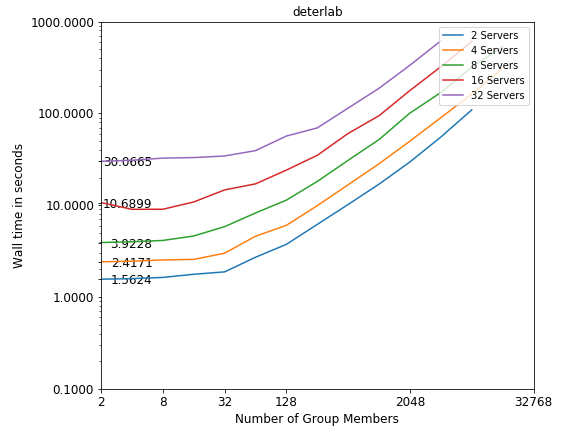
\includegraphics[width=.4\linewidth]{images/plots/authwalltime_deterlab.png} % svg gives me an error
%        }
%        \subfigure[local simulation]{
%            \centering
%            \caption{auth.\ time locally}
%            \label{fig:localauthtime}
%            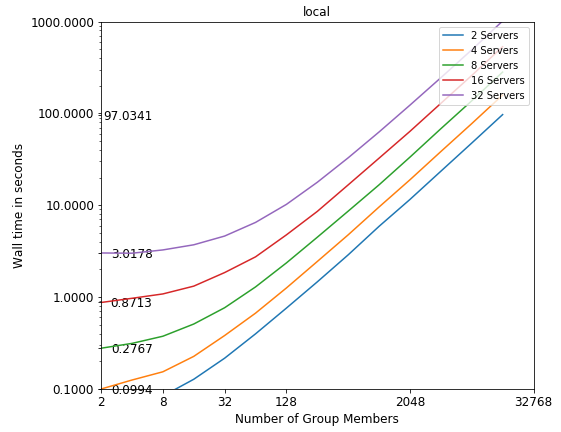
\includegraphics[width=.4\linewidth]{images/plots/authwalltime_local.png}
%        }

%        \begin{subfigure}
%           \centering
%%            \caption{auth.\ time locally}
%%            \label{fig:localauthtime}
%           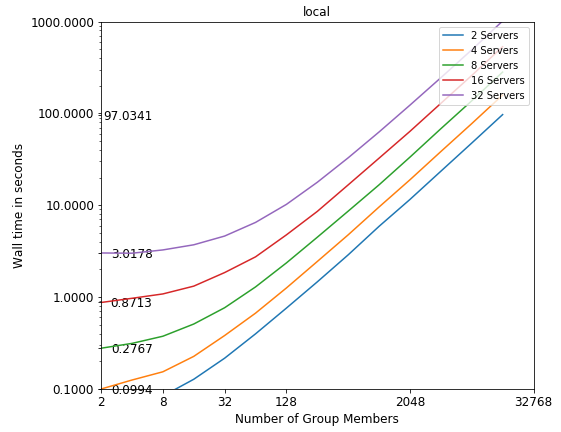
\includegraphics[width=.4\linewidth]{images/plots/authwalltime_local.png}
%        \end{subfigure}
%        \begin{subfigure}
%            \centering
%%            \caption{auth.\ time locally}
%%            \label{fig:localauthtime}
%            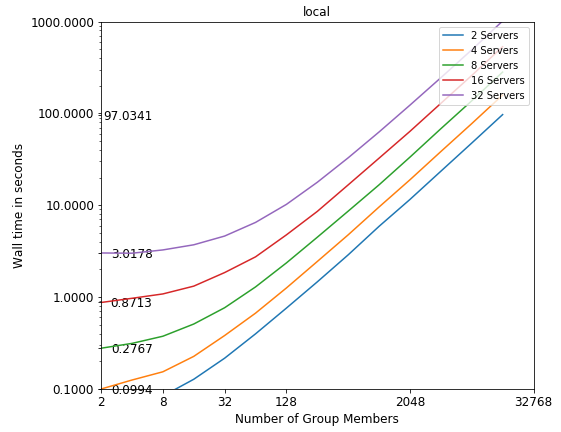
\includegraphics[width=.4\linewidth]{images/plots/authwalltime_local.png}
%        \end{subfigure}
    \begin{figure*}
        \centering
        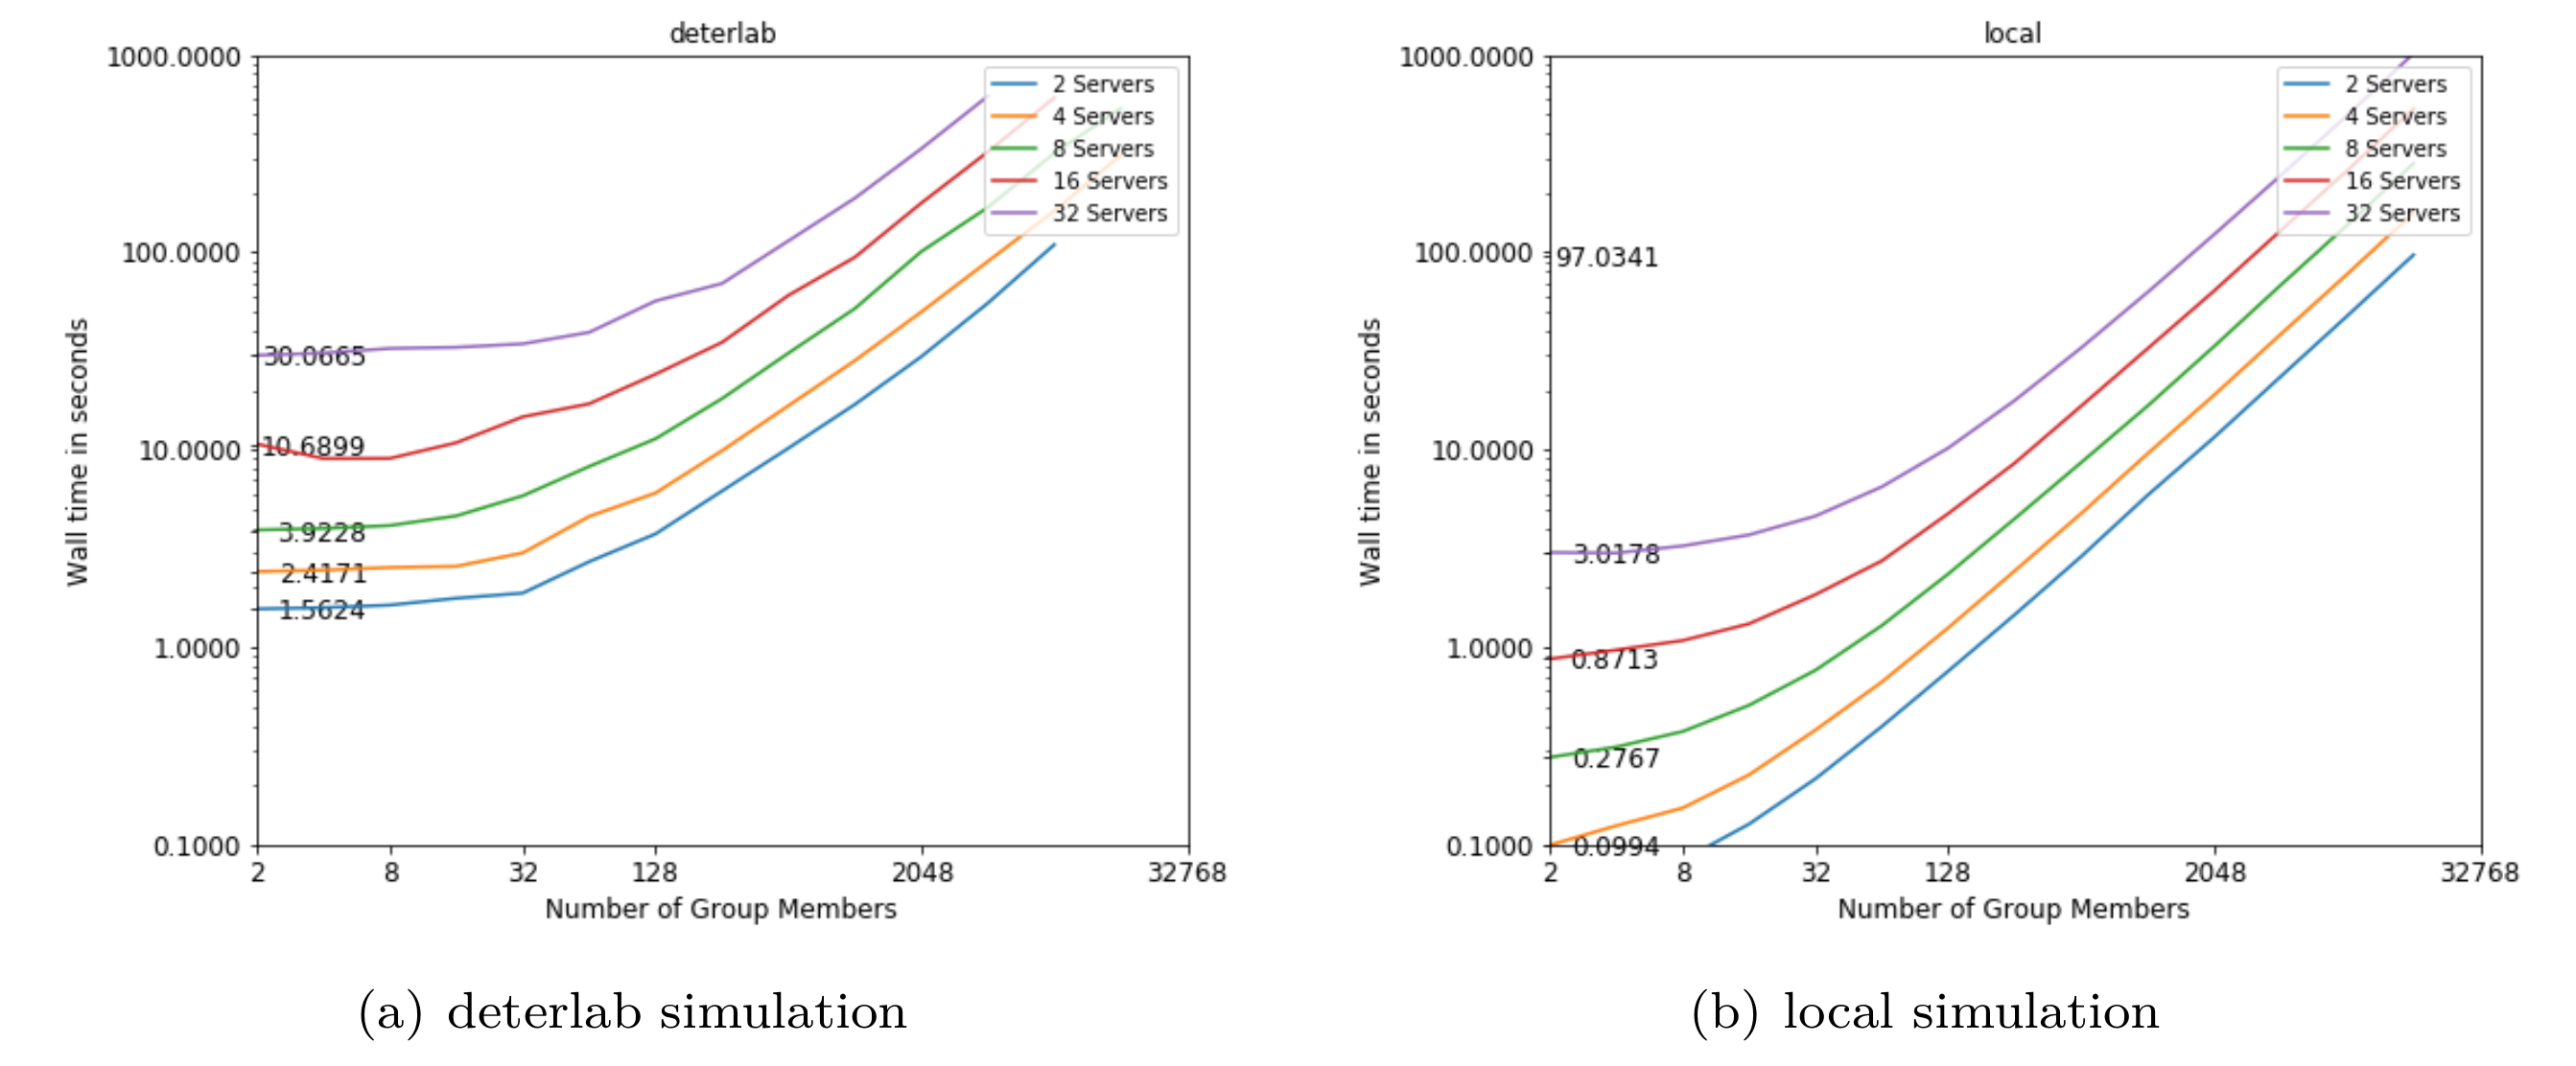
\includegraphics[width=0.8\linewidth]{images/plots/authenticationtimeHack.png}
        \vspace*{1cm}
        \caption{Authentication wall time}
        \label{fig:authtime}
    \end{figure*}
    We can clearly observe the impact of the 100ms delay existing in the DETERLab setting.
    Comparing the results of the local simulation with the one of~\cite{villard_report_pfs_pop.pdf_2017} we can observe
    a small overhead, probably because now we are running a real cothority (overhead of the cothority framework and network communication).
    Hence in all logic when comparing it to the one of~\cite{syta_identity_2015} we notice improvements of the same order
    as the one noticed in~\cite{villard_report_pfs_pop.pdf_2017}.\sidenote{(~10X) for the same reasons, notably moore's law}
    We can see that even when running our simulation in a real world setting (DETERLab) with network delays, we obtain
    authentication times comparable to or only slightly slower than the ones obtained by~\cite{syta_identity_2015}

    \subsubsection{PKClient, Auth, and Total time}

    Fig.~\ref{fig:stackedauthtime}  % FIXME RHAAAAAAAAAAAAAAAAAAAAAA F/*%@# latex wrong fig number !!!!!!!!
    %The following figure
    decompose the total authentication wall time\sidenote{
        Only local simulation shown, in deterlab similar with only difference being that at beginning the 100ms delay dominate
        before becoming insignificant later, same difference as in Fig.~\ref{fig:authtime} above.
    } into the time needed to build the proof (blue) and
    the time needed to process the request (orange).\vspace*{0.3cm}
    \begin{figure*}
        \centering
%        \subfigure[2 servers]{
%            \centering
%            \label{fig:stackedlocal2}
%            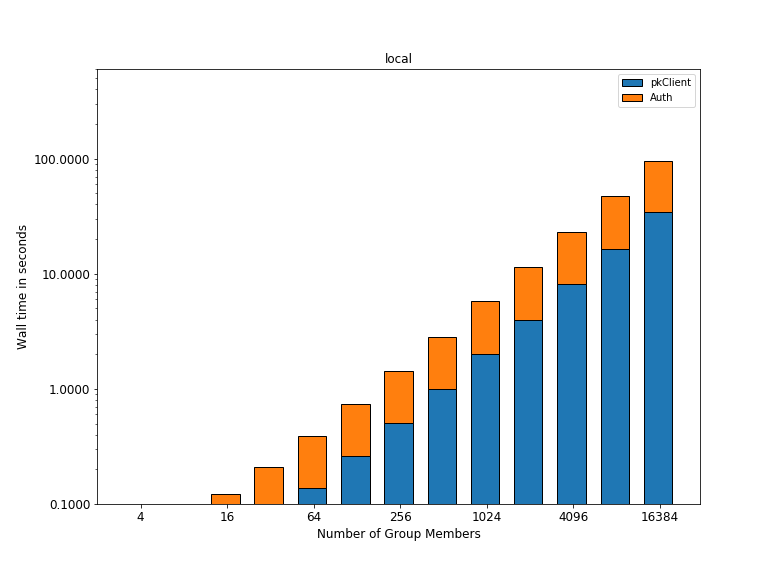
\includegraphics[width=.4\linewidth]{images/plots/stacked2servers_local.png} % svg gives me an error
%        }
%        \subfigure[4 servers]{
%            \centering
%            \label{fig:stackedlocal4}
%            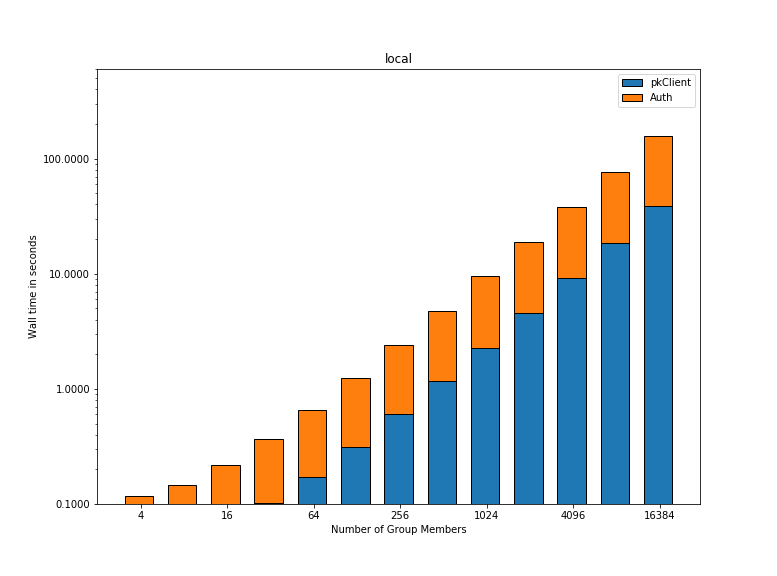
\includegraphics[width=.4\linewidth]{images/plots/stacked4servers_local.png} % svg gives me an error
%        }
%        \subfigure[8 servers]{
%            \centering
%            \label{fig:stackedlocal8}
%            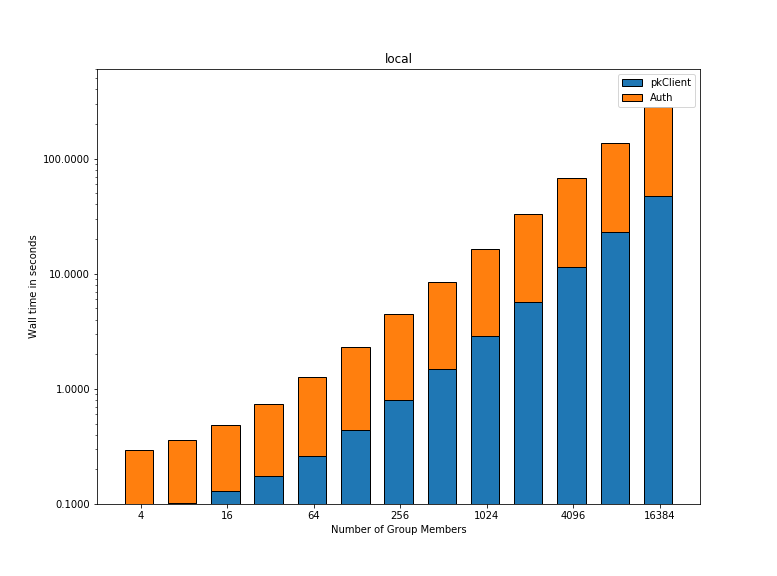
\includegraphics[width=.4\linewidth]{images/plots/stacked8servers_local.png} % svg gives me an error
%        }\newline
%        \subfigure[16 servers]{
%            \centering
%            \label{fig:stackedlocal16}
%            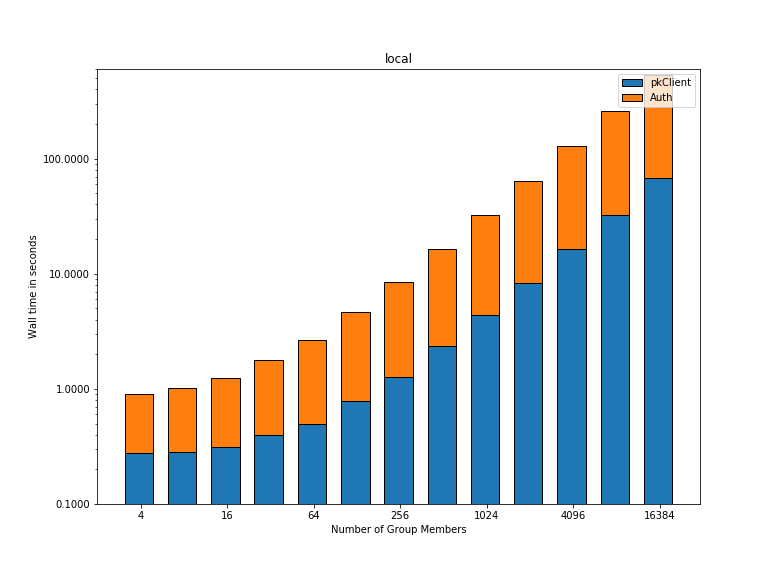
\includegraphics[width=.4\linewidth]{images/plots/stacked16servers_local.png} % svg gives me an error
%        }
%        \subfigure[32 servers]{
%            \centering
%            \label{fig:stackedlocal32}
%            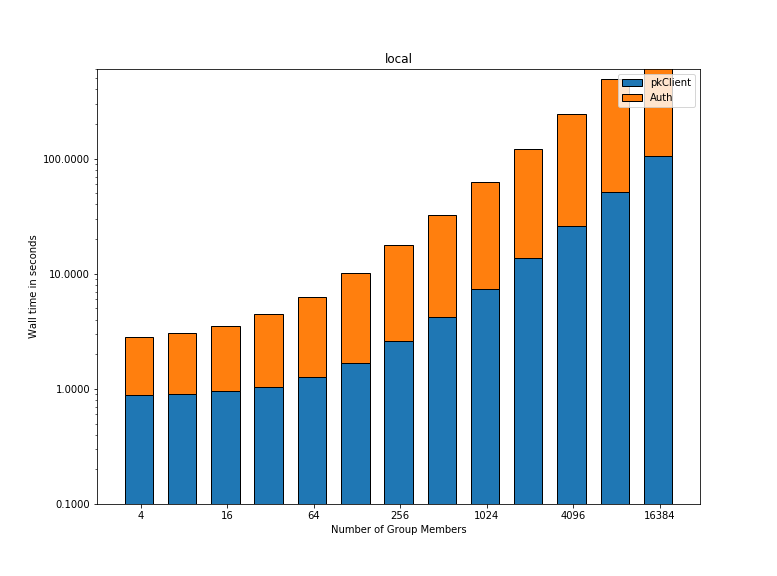
\includegraphics[width=.4\linewidth]{images/plots/stacked32servers_local.png} % svg gives me an error
%        }
        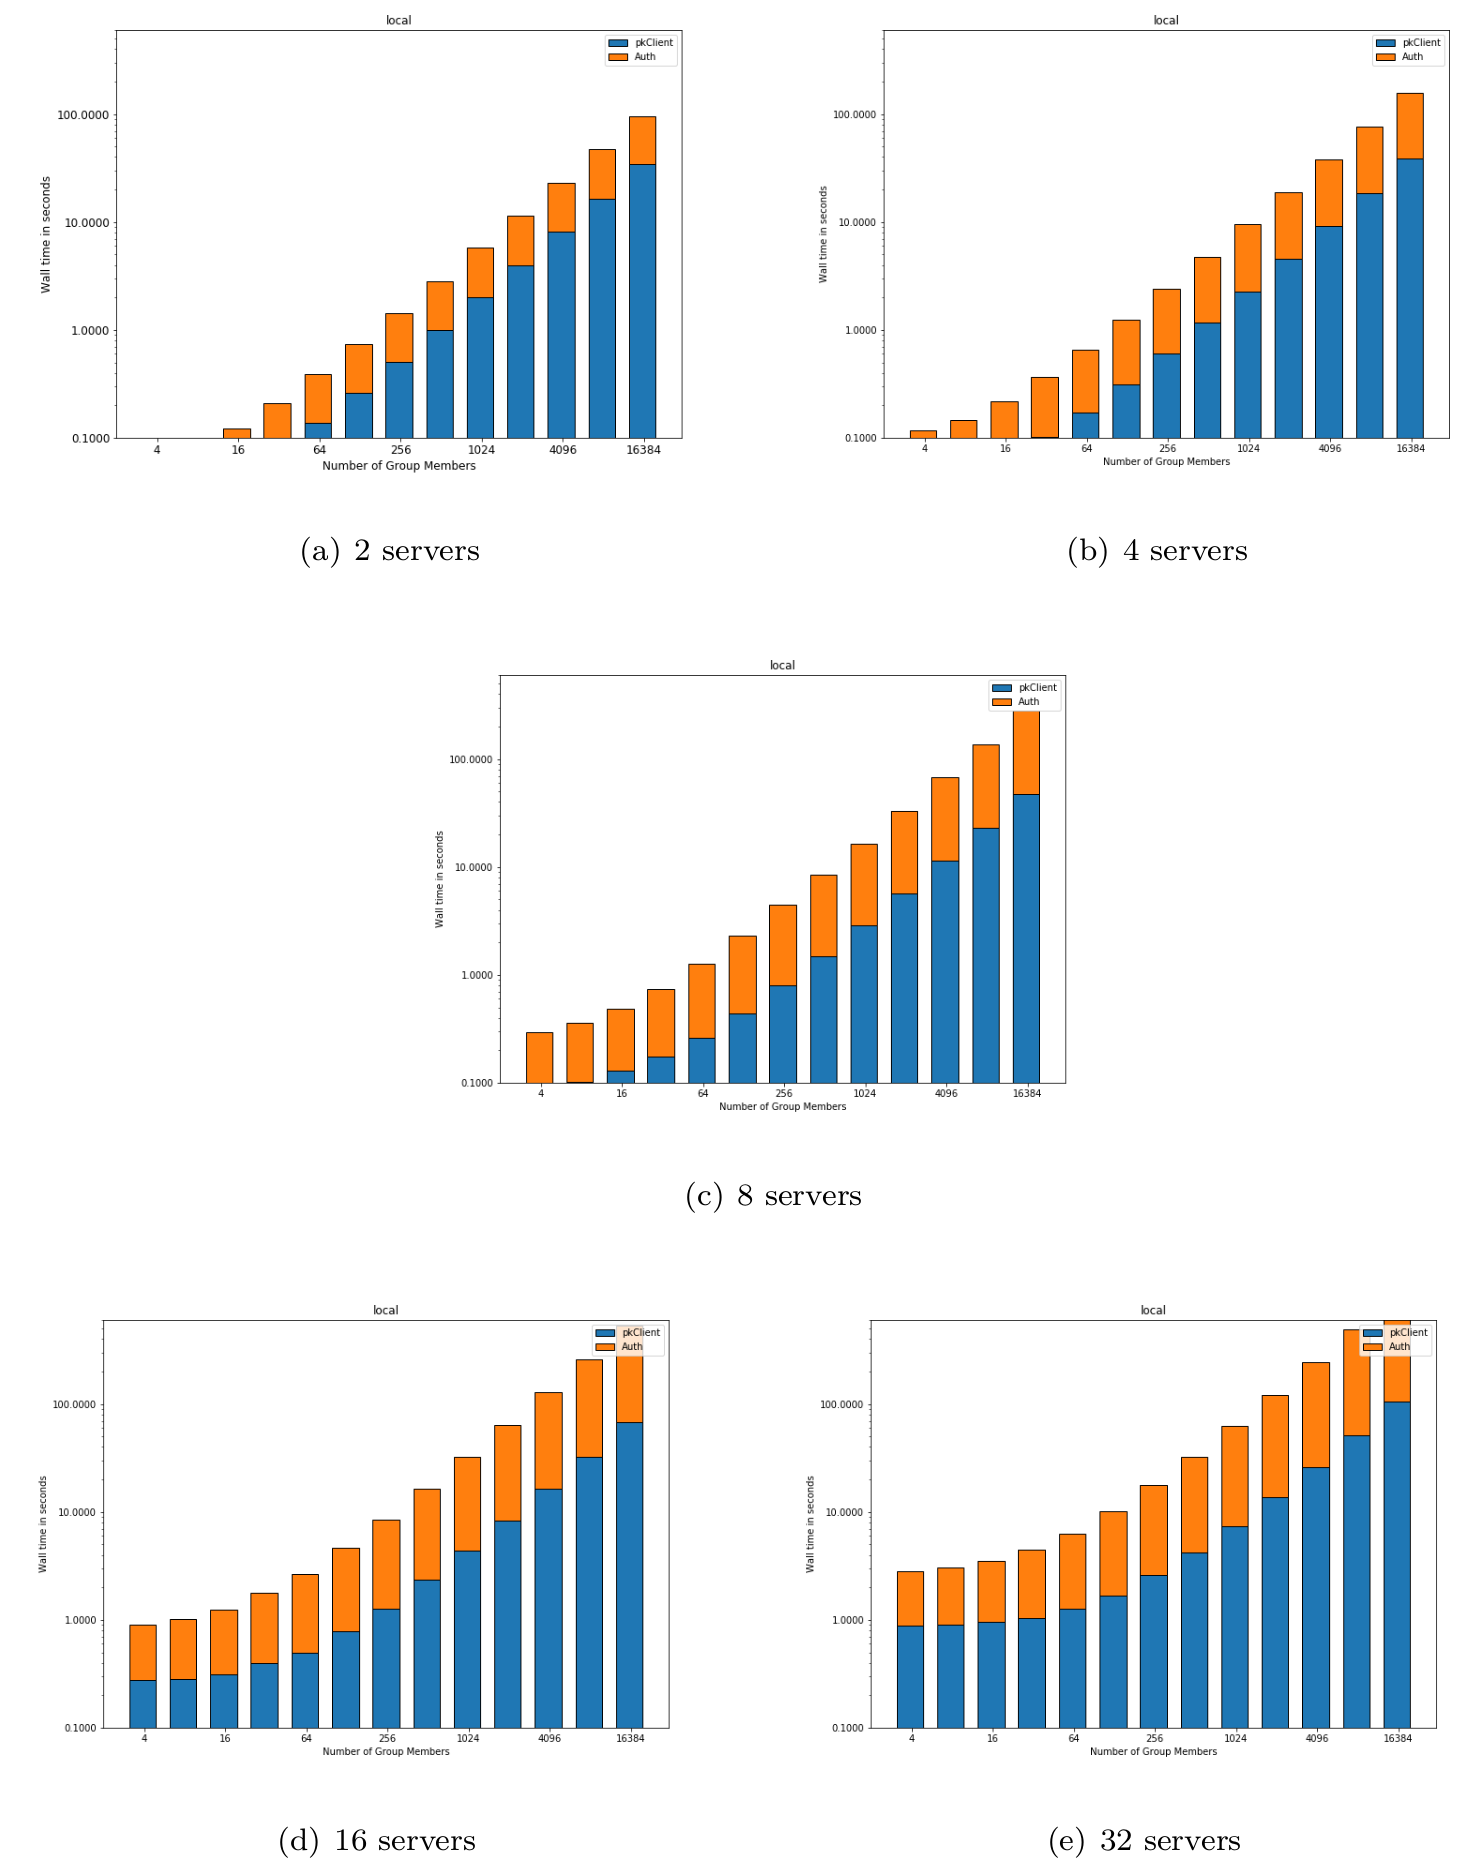
\includegraphics[width=0.8\linewidth]{images/plots/stackedHack.png}
        \vspace*{1cm}
        \caption{Authentication time decomposed}
        \label{fig:stackedauthtime}
    \end{figure*}

    \subsection{Traffic}

    Only the total\sidenote{
        the client-server or server-client traffic should not change much in comparison with~\cite{villard_report_pfs_pop.pdf_2017}.
    } Server traffic was plotted.

    Fig.~\ref{fig:servertraffic} % FIXME RHAAAAAAAAAAAAAAAAAAAAAA F/*%@# latex wrong fig number !!!!!!!!
    %The following figure
    shows the sum of the data sent by each server during the Authentication of a user.

    \begin{figure}
        \centering
        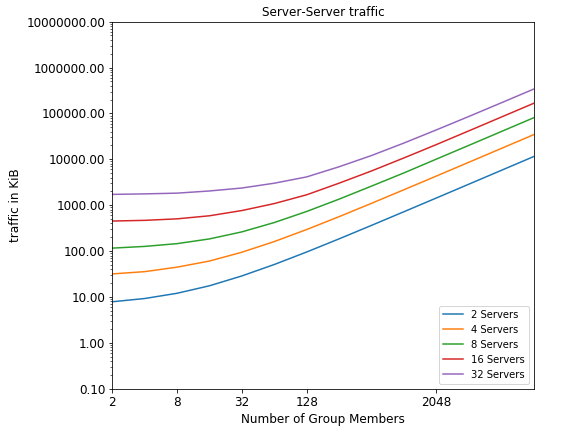
\includegraphics[width=.65\linewidth]{images/plots/serverservertraffic.png} % svg gives me an error
        \vspace*{1cm}
        \caption{Total Server traffic}
        \label{fig:servertraffic}
    \end{figure}

    Finally we share the conclusions that \blockquote{
        all forms of DAGA traffic grow linearly in the number of clients and nearly linearly in the number of servers
    }\cite{syta_identity_2015} hence our results are coherent.

    %TODO ?
    %You can note that there are some holes in the data, that is because we
    % problems : read tcp io timeout, out of memory, ssh keepalive, bug in cothority/onet cache clean/timeout while protocol alive .. ...
    % etc.. etc.. ran short of time and patience


    %the graphs and quick discussion,
    %comment on moore law,
    %say that probably could/should be quicker if X25519 was used (hypothesis, don't make a fool of myself if it is the case)
    %say there are lots of redundant and probably not useful signatures that slowdown everything
    %+ say that coherent with previous implementations


%    \chapter{Future} %and applications and conclusion ?
%    \label{ch:future} :((((

   \chapter{Conclusion}

    This project demonstrates the feasibility of the democratization of DAGA as an anonymous authentication mechanism
    by both \begin{itemize}
        \item allowing  every system able to speak OIDC to make the move (pretty much every system) without pain
        \item and showing that it is possible to offer a user-friendly interface
    \end{itemize}
    This was done without introducing alien ideas into the DAGA library and Cothority making them easier to maintain and reuse for other purposes.
    Nothing prevent us to tie DAGA more closely to the POP framework, everything is already usable, it lacks only the little bit
    of boilerplate extracting the keys from a party transcript.

    Still it is far from being perfect and finished, notably from a "features" point of view, we haven't yet defined ways
    to allow 3rd-party services to evolve the authentication contexts (add / remove users, revoke context, deny authentication if user exhausted some quota of authentication etc.).
    From a security point of view we can list the following things that would need our future attention:
    \begin{itemize}
        \item currently, the authentication messages can be replayed...
        \item we would need ways such as memguard\sidenote{
            https://github.com/awnumar/memguard
        } to protect the storage of secrets and keys in memory.
        \item currently the state of the service contains sensitive information
            (per-round secrets, secret-keys of the daga servers associated with each contexts, etc.)that are persisted into bbolt...
            We propose to make it fully stateless if possible by deriving every needed secret from the master secret key
            of the node and other information and "storing" more state in the clients.
        \item As already said the server-side code of the library would need some reviews too
        \item We noticed that the deniability property as it is currently defined in the paper doesn't totally hold.
            At the end of a successful authentication every servers obtain the list of all the NIZK proofs that state they all did their work correctly.
            Since those proofs are verifiable by anyone and we are in an anytrust setting then for sure someone did authenticate (if not that would mean that
            the honest server did not follow the protocol this could qualify as a dishonest behavior..).
            hence we would need to modify the implementation to periodically add some noise, release proof transcripts that are nothing but simulations etc..
%    this means that we weaken deniability (the NIZK proofs of the servers + anytrust ==> someone authenticated for sure)
%    => in fact even in vanilla daga description if we don't publish the server proofs, at the end of successful auth ALL servers obtain all the proofs and tag
%    => since we are in anytrust mean all but one server can be malicious/dishonnest => deniability doesn't hold as advertised in paper (but still)
    \end{itemize}
%- daga:
%    I took some time investigating if we can keep daga properties (notably deniability) but turn PKClient into a
%    non interactive truly zero knowledge proof or a truly zk proof with a single server.
%    (currently the multiple servers of daga are really only there to satisfy HVZK via anytrust which is here for deniability(and for linkability via the tags..fuck..)
%    and to reduce damages resulting of the compromission of a single server in centralized case,
%    (we cannot tolerate subset of them being down etc..ok we are in a decentralized lab but maybe better to have centralized client server and to have a pool of servers etc..)
%    (NIDA paper, vaudenay construction ONTAP etc..)
%    dropped by lack of time, would be a entire thesis subject and probably very different protocol redo proofs etc..)
%    => since deniability already weakened IMO maybe can think of more efficient ways to guarantee same things but then there are probably already constructs doing the same thing cf vaudenay etc..
%
%    -final goal was not clearly defined
%    at the begining of putting things together was envisioned to use equivalent of pop parties to gather keys as part of the daga/login service
%    (begin - join- end- context generation etc..)


    \bibliographystyle{plainnat} % TODO would like ieeetr but no URL...
    \bibliography{references}
    \chapter{Annex}
    Instructions to run the proof of concept.

    Prerequisites:
    \begin{itemize}
        \item a working Go installation\sidecite{pike_go_nodate}
        \item a working docker and docker-compose installation
        \item retrieve github.com/dedis/student\_18\_daga and install the dagaclient and dagadaemon cli
        \item add the following two aliases to /etc/hosts:\newline
            172.18.0.1 opapp.poc\newline
            172.18.0.1 rpapp.poc\newline
            where 172.18.0.1 should be the IP of your host computer as seen from the future docker containers,
            adapt if it is not the case.
    \end{itemize}

    then:
    \begin{enumerate}
        \item cd in the student\_18\_daga/PoC directory
        \item \emph{make}
        \item follow the instructions on screen
    \end{enumerate}

\end{document}
